\documentclass{article}

% page size and margins
\usepackage[a4paper,top=2cm,bottom=2cm,left=3cm,right=3cm,marginparwidth=1.75cm]{geometry}

% packages
\usepackage{preamble}
\addbibresource{my_biblio.bib} % do not put this in preamble or it breakes automatic suggestions for citations in vscode

% theorems
\newtheorem{theorem}{Theorem}[section]
\newtheorem{corollary}{Corollary}[theorem]
\newtheorem{lemma}[theorem]{Lemma}
\newtheorem{fact}[theorem]{Fact}
\newtheorem{conjecture}[theorem]{Conjecture}
\newtheorem*{theorem*}{Theorem}
\newtheorem*{corollary*}{Corollary}
\newtheorem*{lemma*}{Lemma}
\newtheorem*{fact*}{Fact}
\newtheorem*{conjecture*}{Conjecture}

\theoremstyle{remark}
\newtheorem{remark}{Remark}[section]
\newtheorem*{remark*}{Remark}

\theoremstyle{definition}
\newtheorem{definition}{Definition}[section]
\newtheorem*{definition*}{Definition}

\theoremstyle{definition}
\newtheorem{example}{Example}[section]
\newtheorem*{example*}{Example}

\theoremstyle{definition}
\newtheorem{proposition}{Proposition}[section]
\newtheorem*{proposition*}{Proposition}

% macros
\usepackage{my_macro}
\usepackage{laetitia_macro}

\title{Stage M2}
\author{Davide Ferre'}

\begin{document}

\maketitle

\section{Useful stuff}
\subsection{Message Sequence Charts}

Assume a finite set of processes $\Procs$ and a finite set of messages $\Msg$.
The set of (\pp) channels is $\Ch = \{(p,q) \in \Procs \times \Procs \mid p \neq q\}$.
%
A send action is of the form $\sact{p}{q}{\msg}$
where $(p,q) \in \Ch$ and $\msg \in \Msg$.
It is executed by $p$ and sends message $\msg$ to $q$.
The corresponding receive action, executed by $q$, is
$\ract{p}{q}{\msg}$.
%
For $(p,q) \in \Ch$, let
$\pqsAct{p}{q} = \{\sact{p}{q}{\msg} \mid \msg \in \Msg\}$ and
$\pqrAct{p}{q} = \{\ract{p}{q}{\msg} \mid \msg \in \Msg\}$.
For $p \in \Procs$, we set
$\psAct{p} = \{\sact{p}{q}{\msg} \mid q \in \Procs \setminus \{p\}$ and $\msg \in \Msg\}$, etc.
Moreover, $\pAct{p} = \psAct{p} \cup \qrAct{p}$ will denote the set of all actions that are
executed by $p$.
Finally, $\Act = \bigcup_{p \in \Procs} \pAct{p}$
is the set of all the actions.

\paragraph*{Peer-to-peer MSCs.}
%\alain{add an example of MSC and of system and illustrate notions with it}
A \emph{\pp MSC} (or simply \emph{MSC}) over $\Procs$ and $\Msg$ is a tuple $\msc = (\Events,\procrel,\lhd,\lambda)$
where $\Events$ is a finite (possibly empty) set of \emph{events}
and $\lambda: \Events \to \Act$ is a labeling function.
For $p \in \Procs$, let $\Events_p = \{e \in \Events \mid \lambda(e) \in \pAct{p}\}$ be the set of events
that are executed by $p$.
We require that $\procrel$ (the \emph{process relation}) is the disjoint union $\bigcup_{p \in \Procs} \procrel_p$
of relations ${\procrel_p} \subseteq \Events_p \times \Events_p$ such that
$\procrel_p$ is the direct successor relation of a total order on $\Events_p$.
For an event $e \in \Events$, a set of actions $A \subseteq \Act$, and a relation $\rel \subseteq \Events \times \Events$,
let $\sametype{e}{A}{\rel} = |\{f \in \Events \mid (f,e) \in \rel$ and $\lambda(f) \in A\}|$.
We require that ${\lhd} \subseteq \Events \times \Events$ (the \emph{message relation}) satisfies the following:
\begin{itemize}\itemsep=0.5ex
\item[(1)] for every pair $(e,f) \in {\lhd}$, there is a send action $\sact{p}{q}{\msg} \in \Act$ such that
$\lambda(e) = \sact{p}{q}{\msg}$, $\lambda(f) = \ract{p}{q}{\msg}$, and
$\sametype{e}{\pqsAct{p}{q}}{\procrel^+} = \sametype{f}{\pqrAct{p}{q}}{\procrel^+}$,
\item[(2)] for all $f \in \Events$ such that $\lambda(f)$ is a receive action, there is $e \in \Events$ such that $e \lhd f$.
\end{itemize}
Finally, letting ${\le}_\msc = ({\procrel} \cup {\lhd})^\ast$,
we require that $\le_\msc$ is a partial order. For convenience, we will simply write $\le$ when $M$ is clear from the context. 
%We may also simply write ${\le}$ instead of $\le_{\msc}$ if
%the MSC is clear from the context.

\medskip

Condition (1) above ensures that every (p2p) channel $(p,q)$ behaves in a FIFO manner.
By Condition (2), every receive event has a matching send event.
Note that, however, there may be unmatched send events in an MSC.
We let
$\SendEv{\msc} = \{e \in \Events \mid \lambda(e)$ is a send
action$\}$,
$\RecEv{\msc} = \{e \in \Events \mid \lambda(e)$ is a receive
action$\}$,
$\Matched{\msc} = \{e \in \Events \mid$ there is $f \in \Events$
such that $e \lhd f\}$, and
$\Unm{\msc} = \{e \in \Events \mid \lambda(e)$ is a send
action and there is no $f \in \Events$ such that $e \lhd f\}$.
%
We do not distinguish isomorphic MSCs and
let $\ppMSCs$ be the set of all MSCs over the given sets $\Procs$ and $\Msg$.
% For readability, and if there is no ambiguity,
% $\lambda^{-1}(\send{p}{q}{\msg})$, resp. $\lambda^{-1}(\rec{p}{q}{\msg})$,
% will be written $\ssymb(p,q,\msg)$ and, resp., $\rsymb(p,q,\msg)$ in the examples.

\bigskip

\noindent \begin{minipage}[c]{10.5cm}
  \begin{example}\label{ex:msc}
    For a set of processes $\procSet = \{p,q,r\}$ and a set of messages $\paylodSet = \{\msg_1, \msg_2, \msg_3, \msg_4 \}$,
    $\mscweakuniver = (\Events, \rightarrow, \lhd, \lambda)$
    %in Fig.~\ref{fig:msc_weak_univer}
    is an MSC where, for example,
  $e_2 \lhd e_2'$ and $e_3' \rightarrow e_4$.
  The dashed arrow means that the send event $e_1$ does not have
  a matching receive, so $e_1 \in Unm(\mscweakuniver)$.
  Moreover, $e_2 \le_{\mscweakuniver} e_4$, but
  $e_1 \not\le_{\mscweakuniver} e_4$.
We can find a total order ${\pplin} \supseteq {\le}_{\mscweakuniver}$
  such that $e_1 \pplin e_2 \pplin e_2' \pplin e_3
  \pplin e_3' \pplin e_4 \pplin e_4'$. We call $\pplin$ a linearization,
  which is formally defined  below.
  \end{example}
\end{minipage}
\hfill
\begin{minipage}[c]{3cm}

%\begin{figure}
  \begin{center}
    \begin{tikzpicture}[>=stealth,node distance=3.2cm,shorten >=1pt,
      every state/.style={text=black, scale =0.8}, semithick,
      font={\fontsize{8pt}{12}\selectfont}]
	\begin{scope}[xshift = 9cm, scale = 0.8]
		\node at (-0.3, -0.65)  (e)    {$e_1$};
		\node at (1.3, -1.2)  (e)    {$e_2$};
		\node at (-0.3, -1.2)  (e)    {$e_2'$};
		\node at (0.7, -1.85)  (e)    {$e_3$};
		\node at (2.3, -1.85)  (e)    {$e_3'$};
		\node at (2.3, -2.4)  (e)    {$e_4$};
		\node at (0.7, -2.4)  (e)    {$e_4'$};
		%MACHINES
		\draw (0,0) node{$p$} ;
		\draw (1,0) node{$q$} ;
		\draw (2,0) node{$r$} ;
		\draw (0,-0.2) -- (0,-2.8) ;
		\draw (1,-0.2) -- (1,-2.8);
		\draw (2, -0.2) -- (2, -2.8) ;
		%MESSAGES
		\draw[>=latex,->, dashed] (0,-0.65) -- (1, -0.65) node[midway,above]{$\amessage_1$};

		\draw[>=latex,->] (1, -1.2) -- (0, -1.2) node[midway, above] {$\amessage_2$};

		\draw[>=latex,->] (1,-1.85) -- (2,-1.85) node[midway, above] {$\amessage_3$};

		\draw[>=latex,->] (2,-2.4) -- (1,-2.4) node[midway,above] {$\amessage_4$};
	\end{scope}

\end{tikzpicture}
\captionof{figure}{MSC $\mscweakuniver$}
\label{fig:msc_weak_univer}
\end{center}
%\alain{NIce}
%\end{figure}

\end{minipage}

\paragraph*{Mailbox MSCs.}

For an MSC $\msc = (\Events,\procrel,\lhd,\lambda)$, we define
an additional binary relation that represents a constraint
under the mailbox semantics, where each process has only one incoming channel.
Let ${\mbrel}_\msc \subseteq \Events \times \Events$
be defined by: $e_1 \mbrel_\msc e_2$ if there is $q \in \Procs$
such that $\lambda(e_1) \in \qsAct{q}$,
$\lambda(e_2) \in \qsAct{q}$, and one of the following holds:
\begin{itemize}\itemsep=0.5ex
\item $e_1 \in \Matched{\msc}$ and $e_2 \in \Unm{\msc}$, or
\item $e_1 \lhd f_1$ and $e_2 \lhd f_2$ for some $f_1,f_2 \in \Events_q$ such that $f_1 \procrel^+ f_2$.
\end{itemize}

We let ${\preceq_\msc} = ({\procrel} \,\cup\, {\lhd} \,\cup\, {\mbrel_\msc})^\ast$.
Note that ${\le_\msc} \subseteq {\preceq_\msc}$.
%
%\begin{definition}\label{def:mailbox-msc}
We call $\msc \in \ppMSCs$ a \emph{mailbox MSC}
if ${\preceq_\msc}$ is a partial order.
%\end{definition}
Intuitively, this means that events can be scheduled in a way that corresponds
to the mailbox semantics, i.e., with one incoming channel per process.
Following the terminology in \cite{DBLP:conf/cav/BouajjaniEJQ18}, we also say that
a mailbox MSC satisfies \emph{causal delivery}.
The set of mailbox MSCs $\msc \in \ppMSCs$ is denoted by $\cdMSCs$.

\begin{example}\label{ex:mailbox-msc}
    MSC $\mscweakuniver$ is a mailbox MSC. Indeed, even though the order $\linrel$ defined in Example~\ref{ex:msc} does not respect all mailbox constraints, particularly the fact that $e_4 \mbrel_{\mscweakuniver} e_1$, there is a total order $ {\mblin} \supseteq {\preceq_{\mscweakuniver}}$ such that $
    e_2 \mblin e_3 \mblin e_3' \mblin e_4 \mblin e_1 \mblin e_2' \mblin e_4'$. We call $\mblin$ a mailbox linearization, which is formally defined below.
\end{example}

\paragraph*{Linearizations, Prefixes, and Concatenation.}

Consider $\msc = (\Events,\procrel,\lhd,\lambda) \in \MSCs$.
A \emph{\pp linearization} (or simply \emph{linearization}) of $\msc$ is a (reflexive) total order
${\linrel} \subseteq \Events \times \Events$ such that ${\le_\msc} \subseteq
{\linrel}$. Similarly,
a \emph{mailbox linearization} of $\msc$ is a total order
${\linrel} \subseteq \Events \times \Events$ such that ${\preceq_\msc} \subseteq
{\linrel}$. That is, every mailbox linearization is a \pp linearization,
but the converse is not necessarily true (Example~\ref{ex:mailbox-msc}).
Note that an MSC is a mailbox MSC iff it has at least one mailbox linearization.

\medskip

Let $\msc = (\Events,\procrel,\lhd,\lambda) \in \MSCs$ and consider
$E \subseteq \Events$ such that $E$ is ${\le_\msc}$-\emph{downward-closed}, i.e,
for all $(e,f) \in {\le_\msc}$ such that $f \in E$, we also have $e \in E$.
Then, the MSC $(E,{\procrel} \cap (E \times E),{\lhd} \cap (E \times E),\lambda')$,
where $\lambda'$ is the restriction of $\Events$ to $E$, is called a \emph{prefix}
of $\msc$. In particular, the empty MSC is a prefix of $\msc$.
We denote the set of prefixes of $\msc$ by $\Pref{\msc}$.
This is extended to sets $L \subseteq \MSCs$ as expected, letting
$\Pref{L} = \bigcup_{\msc \in L} \Pref{\msc}$.

\begin{lemma}
\label{lem:mb-prefix}
Every prefix of a mailbox MSC is a mailbox MSC.
\end{lemma}
\begin{proof}
Let $\msc = (\Events, \procrel, \lhd, \lambda) \in \mbMSCs$ and $\msc_0 =
(\Events_0, \procrel_0, \lhd_0, \lambda_0)$ be a prefix of $\msc$, i.e.,
$\Events_0 \subseteq \Events$. By contradiction, suppose that $\msc_0$ is not a
mailbox MSC. Then, there are distinct $e,f \in \Events_0$ such that $e \preceq_{M_0} f \preceq_{M_0}
e$ with ${\preceq_{\msc_0}} = ({\rightarrow_0} \cup {\lhd_0} \cup {\mbrel_{\msc_0}})^*$.
As $\Events_0 \subseteq \Events$, we have that ${\rightarrow_0} \subseteq {\rightarrow}$, ${\lhd_0} \subseteq {\lhd}$, and ${\mbrel_{\msc_0}} \subseteq {\mbrel_{\msc}}$. Finally, ${\preceq_{\msc_0}} \subseteq {\preceq_{\msc}}$ and $\msc$ is not a mailbox MSC, which is a contradiction.
\end{proof}

Let $\msc_1 = (\Events_1,\procrel_1,\lhd_1,\lambda_1)$ and
$\msc_2 = (\Events_2,\procrel_2,\lhd_2,\lambda_2)$ be two MSCs.
Their \emph{concatenation} $\msc_1 \cdot \msc_2 = (\Events,\procrel,\lhd,\lambda)$ is defined if, for all $(p,q) \in \Ch$,
$e_1 \in \Unm{\msc_1}$, and
$e_2 \in \Events_2$ such that $\lambda(e_1) \in \pqsAct{p}{q}$
and $\lambda(e_2) \in \pqsAct{p}{q}$,
we have $e_2 \in \Unm{\msc_2}$.
As expected, $\Events$ is the disjoint union of $\Events_1$ and $\Events_2$,
${\lhd}  = {\lhd_1} \cup {\lhd_2}$, $\lambda$ is the ``union'' of $\lambda_1$
and $\lambda_2$, and ${\procrel} = {\procrel_1} \cup {\procrel_2} \cup R$.
Here, $R$ contains, for all $p \in \Procs$ such that $(\Events_1)_p$ and
$(\Events_2)_p$ are non-empty, the pair $(e_1,e_2)$ where $e_1$ is the
maximal $p$-event in $M_1$ and $e_2$ is the minimal $p$-event in $M_2$.
Note that $\msc_1 \cdot \msc_2$ is indeed an MSC and that
concatenation is associative.

\subsection{Communicating Systems}

We now recall the definition of communicating systems (aka communicating finite-state
machines or message-passing automata), which consist of finite-state machines $A_p$
(one for every process $p \in \Procs$) that can communicate through the FIFO channels
from $\Ch$.

\begin{definition}\label{def:cs}
A \emph{communicating system} over $\Procs$ and $\Msg$ is a tuple
   $ \Sys = (A_p)_{p\in\procSet}$. For each
   $p \in \Procs$, $A_p = (Loc_p, \delta_p, \ell^0_p)$ is a finite transition system where
   $\Loc_p$ is a finite set of local (control) states, $\delta_p
   \subseteq \Loc_p \times \pAct{p} \times \Loc_p$ is the
   transition relation, and $\ell^0_p \in Loc_p$ is the initial state.
\end{definition}

Given $p \in \Procs$ and a transition $t = (\ell,a,\ell') \in \delta_p$, we let
$\tsource(t) = \ell$, $\ttarget(t) = \ell'$, $\tlabel(t) = a$, and
$\tmessage(t) = \msg$ if $a \in \msAct{\msg} \cup \mrAct{\msg}$.

\smallskip

There are in general two ways to define the semantics of a communicating system.
Most often it is defined as a global infinite transition system that keeps track
of the various local control states and all (unbounded) channel contents.
As, in this paper, our arguments are based on a graph view of MSCs, we will define
the language of $\Sys$ directly as a set of MSCs. These two semantic views are essentially
equivalent, but they have different advantages depending on the context.
We refer to \cite{CyriacG14} for a thorough discussion.

Let $\msc = (\Events,\procrel,\lhd,\lambda)$ be an MSC.
A \emph{run} of $\Sys$ on $\msc$ is a mapping
$\rho: \Events \to \bigcup_{p \in \Procs} \delta_p$
that assigns to every event $e$ the transition $\rho(e)$
that is executed at $e$. Thus, we require that
\begin{enumerate*}[label={(\roman*)}]
\item for all $e \in \Events$, we have $\tlabel(\rho(e)) = \lambda(e)$,
\item for all $(e,f) \in {\procrel}$, $\ttarget(\rho(e)) = \tsource(\rho(f))$,
\item for all $(e,f) \in {\lhd}$, $\tmessage(\rho(e)) = \tmessage(\rho(f))$,
and
\item for all $p \in \Procs$ and $e \in \Events_p$ such that there is no $f \in \Events$ with $f \procrel e$, we have $\tsource(\rho(e)) = \ell_p^0$.
\end{enumerate*}

Letting run $\Sys$ directly on MSCs is actually very convenient.
This allows us to associate with $\Sys$ its p2p language and mailbox language
in one go. The \emph{\pp language} of $\Sys$ is $\ppL{\Sys} = \{\msc \in \ppMSCs \mid$ there is a run of $\Sys$ on $\msc\}$.
The \emph{mailbox language} of $\Sys$ is $\mbL{\Sys} = \{\msc \in \mbMSCs \mid$ there is a run of $\Sys$ on $\msc\}$.

Note that, following \cite{DBLP:conf/cav/BouajjaniEJQ18,DBLP:conf/fossacs/GiustoLL20},
we do not consider final states or final configurations, as our purpose is to
reason about all possible
traces that can be \emph{generated} by $\Sys$.
%We will discuss this issue in more detail later in the paper. \todo{Do we still discuss this in the conference version or can we omit this sentence?}
The next lemma is obvious for the p2p semantics and follows from Lemma~\ref{lem:mb-prefix} for
	the mailbox semantics.

\begin{lemma}\label{lem:prefix-closed}
For all $\comsymb \in \{\ppsymb, \mbsymb\}$, $\cL{\Sys}$ is prefix-closed:
$\Pref{\cL{\Sys}} \subseteq \cL{\Sys}$.
\end{lemma}

\begin{example}
	Fig.~\ref{fig:system_weak_univer} depicts $\systemweakuniver = (A_p, A_q, A_r)$ such that MSC $\mscweakuniver$ in Fig.~\ref{fig:msc_weak_univer} belongs to $\ppL{\systemweakuniver}$ and to $\mbL{\systemweakuniver}$.
	There is a unique run $\rho$ of $\systemweakuniver$ on $\mscweakuniver$.
	We can see that $(e_3',e_4) \in {\rightarrow}$ and $\ttarget(\rho(e_3')) = \tsource(\rho(e_4)) = \ell_r^{1}$, $(e_2, e_2') \in \lhd_{\mscweakuniver}$, and $\tmessage(\rho(e_2)) = \tmessage(\rho(e_2')) = \msg_2$.
	\end{example}
	\begin{figure}[t]
	\begin{center}
	  \begin{tikzpicture}[>=stealth,node distance=3.2cm,shorten >=1pt,
		every state/.style={text=black, scale =0.75}, semithick,
		font={\fontsize{8pt}{12}\selectfont},
		scale = 0.9
		]
	  \begin{scope}[->]
		  \node[state,initial,initial text={}] (q0)  {$\ell_p^{0}$};
		  \node[state, right of=q0] (q1)  {$\ell_p^{1}$};
				\node[state, right of=q1] (q2) {$\ell_p^{2}$};
	
			\path (q0) edge node [above] {$\send{p}{q}{\msg_1}$} (q1);
				\path (q1) edge node [above] {$\rec{q}{p}{\msg_2}$}(q2);
			\node[thick] at (-1.1,0) {$A_p$};
	  \end{scope}
	
	  \begin{scope}[->, shift={(7.5,0)}]
		  \node[state,initial,initial text={}] (q0)  {$\ell_q^{0}$};
				\node[state, right of=q0] (q1)  {$\ell_q^{1}$};
				\node[state, below of=q1, node distance = 1.5cm] (q2) {$\ell_q^{2}$};
				\node[state, left of=q2] (q3)  {$\ell_q^{3}$};
	
				\path (q0) edge node [above] {$\send{q}{p}{\msg_2}$} (q1);
				\path (q1) edge node [right] {$\send{q}{r}{\msg_3}$}(q2);
				\path (q2) edge node [above] {$\rec{r}{q}{\msg_4}$} (q3);
				\node[thick] at (-1.1,0) {$A_q$};
	  \end{scope}
	
		\begin{scope}[->, shift={(0,-1.25)} ]
		  \node[state,initial,initial text={}] (q0)  {$\ell_r^{0}$};
				\node[state, right of=q0] (q1)  {$\ell_r^{1}$};
				\node[state, right of=q1] (q2) {$\ell_r^{2}$};
	
				\path (q0) edge node [above] {$\rec{q}{r}{\msg_3}$} (q1);
				\path (q1) edge node [above] {$\send{r}{q}{\msg_4}$}(q2);
				\node[thick] at (-1.1,0) {$A_r$};
	  \end{scope}
	\end{tikzpicture}
	\captionof{figure}{System $\systemweakuniver$}
	\label{fig:system_weak_univer}
	\end{center}
	\end{figure}	

\subsection{Conflict Graph}

We now recall the notion of a conflict graph associated to an MSC defined in \cite{DBLP:conf/cav/BouajjaniEJQ18}. This graph is used to depict the causal dependencies between message exchanges.  Intuitively, we have a dependency whenever
two messages have a process in common. For instance, an $\xrightarrow{SS}$
dependency between message exchanges $v$ and $v'$ expresses the fact that
$v'$ has been sent after $v$, by the same process. This notion is of interest because it was seen in \cite{DBLP:conf/cav/BouajjaniEJQ18} that the notion of synchronizability in MSCs (which is studied in this paper) can be graphically characterized by the nature of the associated conflict graph.
It is defined in terms of linearizations
in \cite{DBLP:conf/fossacs/GiustoLL20}, but we equivalently express it
directly in terms of MSCs.

\newcommand{\type}{\tau}
\newcommand{\stype}{S}
\newcommand{\rtype}{R}
\newcommand{\mexch}{\mu}
\newcommand{\Edges}{\mathit{Edges}}
\newcommand{\Nodes}{\mathit{Nodes}}

For an MSC $\msc = (\Events, \rightarrow, \lhd, \lambda)$ and
$e \in \Events$, we define the type $\type(e) \in \{\stype,\rtype\}$ of $e$ by $\type(e) = \stype$ if $e \in \SendEv{\msc}$
and $\type(e) = \rtype$ if $e \in \RecEv{\msc}$.
Moreover, for $e \in \Unm{\msc}$, we let $\mexch(e) = e$,
and for $(e,e') \in \lhd$, we let $\mexch(e) = \mexch(e') = (e,e')$.


\begin{definition}[Conflict graph]
	The \emph{conflict graph} $\cgraph{\msc}$ of an MSC $\msc = (\Events, \rightarrow, \lhd, \lambda)$ is the labeled graph $(\Nodes, \Edges)$, with $\Edges \subseteq \Nodes \times \{\stype,\rtype\}^2 \times \Nodes$, defined by
	$\Nodes = {\lhd} \cup \Unm{\msc}$ and $\Edges = \{(\mu(e),\type(e)\type(f),\mu(f)) \mid (e,f) \in {\to^+}\}$.
In particular, a node of $\cgraph{\msc}$ is either a single unmatched send event or a message pair $(e,e') \in {\lhd}$.
\end{definition}	

\subsection{Logic and Special Tree-Width}

\paragraph*{Monadic Second-Order Logic.}
The set of MSO formulas over MSCs (over $\Procs$ and $\Msg$) is given by the grammar
$
\phi ::= x \procrel y \mid x \lhd y \mid \lambda(x) = a \mid x = y \mid x \in X \mid \exists x.\phi \mid \exists X.\phi \mid \phi \vee \phi \mid \neg \phi
$,
where $a \in \Act$, $x$ and $y$ are first-order variables, interpreted as
events of an MSC, and $X$ is a second-order variable, interpreted
as a set of events. We assume that we have an infinite supply of variables,
and we use common abbreviations such as $\wedge$, $\forall$, etc.
The satisfaction relation is defined in the standard way and self-explanatory.
For example, the formula $\neg\exists x.(\bigvee_{a \in \sAct} \lambda(x) = a \;\wedge\; \neg \mathit{matched}(x))$
with $\mathit{matched}(x) = \exists y.x \lhd y$
says that there are no unmatched send events.
It is not satisfied by  MSC $\mscweakuniver$
of Fig.~\ref{fig:msc_weak_univer},
as message $\msg_1$ is not received,
but by $\mscstrongexist$ from Fig.~\ref{fig:msc_strong_exist}.

Given a sentence $\phi$, i.e., a formula without free variables,
we let $L(\phi)$ denote the set of (p2p) MSCs that satisfy $\phi$.
%
It is worth mentioning that the (reflexive) transitive closure of
a binary relation defined by an MSO formula with free variables $x$ and $y$,
such as $x \procrel y$, is MSO-definable so that the logic can freely
use formulas of the form $x \procrel^+ y$ or $x \le y$ (where $\le$
is interpreted as $\le_\msc$ for the given MSC $\msc$).
Therefore, the definition of a mailbox MSC can be readily translated into
the formula $\mbformula = \neg \exists x.\exists y.(\neg (x = y) \wedge x \preceq y \wedge y \preceq x)$ so that we have $L(\mbformula) = \mbMSCs$.
Here, $x \preceq y$ is obtained as the MSO-definable reflexive transitive closure of
the union of the MSO-definable relations $\procrel$, $\lhd$, and $\sqsubset$.
In particular, we may define $x \sqsubset y$ by :
\[
x \sqsubset y =
\displaystyle
\hspace{-1em}\bigvee_{\substack{q \in \Procs\\a,b \in \qsAct{q}}}\hspace{-1em}
\lambda(x) = a \;\wedge\; \lambda(y) = b
\wedge
\left(
\begin{array}{rl}
& \mathit{matched}(x) \wedge \neg \mathit{matched}(y)\\[1ex]
\vee & \exists x'.\exists y'. (x \lhd x' \;\wedge\; y \lhd y' \;\wedge\; x' \procrel^+ y')
\end{array}
\right)
\]

\paragraph*{Special Tree-Width.}

\emph{Special tree-width} \cite{Courcelle10},
is a graph measure that indicates how close
a graph is to a tree (we may also use classical
	\emph{tree-width} instead).
This or similar measures are commonly employed in verification. For instance, tree-width and split-width have been used in \cite{MadhusudanP11} and, respectively, \cite{DBLP:conf/concur/CyriacGK12,AiswaryaGK14} to reason about graph behaviors generated by pushdown and queue systems.
%Here we apply it to reason about MSCs.
There are several ways to define the special tree-width of an MSC.
We adopt the following game-based definition from \cite{DBLP:journals/corr/abs-1904-06942}.

Adam and Eve play a two-player turn based ``decomposition game''
whose positions
are MSCs with some pebbles placed on some events.
More precisely, Eve's positions are
\emph{marked MSC fragments} $(M, U)$, where
$\msc = (\Events, \procrel, \lhd, \lambda)$
is an \emph{MSC fragment} (an MSC with possibly some edges from
$\lhd$ or $\to$ removed)
 and $U \subseteq \Events$ is the subset of marked events.
Adam's positions are pairs of marked MSC fragments.
A move by Eve consists in the following steps:
\begin{enumerate}
	\item marking some events of the MSC resulting in $(M, U')$ with $U \subseteq U' \subseteq \Events$,
	\item removing (process and/or message) edges whose endpoints are marked,
	\item dividing $(M, U)$ in $(M_1, U_1)$ and $(M_2, U_2)$ such that $M$ is the disjoint (unconnected) union of $M_1$ and $M_2$
	and marked nodes are inherited.
\end{enumerate}
When it is Adam's turn, he simply chooses one of the two marked MSC fragments.
The initial position is $(\msc,\emptyset)$ where $M$ is the (complete) MSC at hand. A terminal position is any position belonging to Eve such that all events are marked.
%
For $k \in \N$, we say that the game is $k$-winning for Eve if she has a (positional) strategy that allows her,
starting in the initial position and independently of Adam's moves, to reach a terminal position such that, in every single position visited along the play, there are at most $k+1$ marked events.

\newcommand{\CS}[2]{\mathsf{CS}_{(#1,#2)}}
\newcommand{\MSO}[2]{\mathsf{MSO}_{(#1,#2)}}
\newcommand{\LCPDL}[2]{\mathsf{LCPDL}_{(#1,#2)}}
\newcommand{\MSCpm}[2]{\mathsf{MSC}_{(#1,#2)}}
\newcommand{\mbMSCpm}[2]{\mathsf{MSC}_{(#1,#2)}^{\mathsf{mb}}}


\begin{fact}[\cite{DBLP:journals/corr/abs-1904-06942}]
	The special tree-width of an MSC is the least $k$ such that
	the associated game is $k$-winning for Eve.
\end{fact}

The set of MSCs whose special tree-width is at most $k$ is denoted by $\stwMSCs{k}$.

\subsection{Model Checking}

In general, even simple verification problems, such
as control-state reachability, are undecidable for
communicating systems \cite{DBLP:journals/jacm/BrandZ83}.
However, they are decidable when we restrict to behaviors of
bounded special tree-width, which motivates the following
definition of a generic {\bf bounded model-checking problem} for $\comsymb \in \{\ppsymb, \mbsymb\}$:\\
%
{\bf Input:} Two finite sets $\Procs$ and $\Msg$, a communicating system $\System$, an MSO sentence $\phi$, and $k \in \N$ (given in unary).\\
%
{\bf Question:} Do we have $\cL{\Sys} \cap \stwMSCs{k} \subseteq L(\phi)$?


\begin{fact}[\cite{DBLP:journals/corr/abs-1904-06942}]\label{p2p}
The bounded model-checking problem for $\comsymb = \ppsymb$ is decidable.
When the formulas $\phi$ are from LCPDL, then the problem is solvable
in exponential time.
\end{fact}

Note that \cite{DBLP:journals/corr/abs-1904-06942} does not employ
the LCPDL modality $\jump$, but it can be integrated easily.
Using $\mbformula$ or $\mbFormula$, we obtain the corresponding result
for mailbox systems as a corollary:
% (cf.\ Appendix~\ref{app:mailbox} for the proof):

\begin{theorem}
\label{thm:mailbox_bounded_model_checking}
The bounded model-checking problem for $\comsymb =  \mbsymb$ is decidable.
When the formulas $\phi$ are from LCPDL, then the problem is solvable
in exponential time.
\end{theorem}

\subsection{Synchronizability}

The above model-checking approach is incomplete in the sense that
a positive answer does not imply correctness of the whole
system. The system may still produce behaviors of special tree-width greater than $k$
that violate the given property.
However, if we know that a system only generates
behaviors from a class whose special tree-width is bounded by $k$,
we can still conclude that the system is correct.

This motivates the \emph{synchronizability problem}.
Several notions of synchronizability have been introduced in the literature.
However, they all amount to asking whether all behaviors generated by
a given communicating system have a particular shape,
i.e., whether they are all included in a fixed (or given) set of MSCs $\Class$.
Thus, the synchronizability problem is essentially an inclusion problem,
namely $\ppL{\Sys} \subseteq \Class$ or $\mbL{\Sys} \subseteq \Class$.
%
We show that, for decidability, it is enough to have that $\Class$
is MSO-definable and special-tree-width-bounded (STW-bounded):
%
We call $\Class \subseteq \MSCs$
\begin{enumerate*}[label={(\roman*)}]
\item \emph{MSO-definable} if there is
an MSO-formula $\phi$ such that $L(\phi) = \Class$,
\item \emph{LCPDL-definable} if there is an
an LCPDL-formula $\Phi$ such that $L(\Phi) = \Class$,
\item \emph{STW-bounded} if there is $k \in \N$
such that $\Class \subseteq \stwMSCs{k}$.
%\item \emph{\nameclass} if it is MSO-definable and STW-bounded.
\end{enumerate*}

An important component of the decidability proof is the following lemma,
which shows that we can reduce synchronizability
wrt.\ an STW-bounded class to bounded model-checking.

\begin{lemma}\label{lem:continuous}
Let $\System$ be a communicating system, $\comsymb \in \{\ppsymb, \mbsymb\}$,
$k \in \N$, and $\Class \subseteq \stwMSCs{k}$.
Then, $\cL{\System} \subseteq \Class$ iff
$\cL{\System} \cap \stwMSCs{(k+2)} \subseteq \Class$.
\end{lemma}

The result follows from the following lemma.
%, whose proof is in Appendix~\ref{app:continuous2}.
Note that a similar property
was shown in \cite[Proposition~5.4]{GKM07} for the specific class of existentially
$k$-bounded MSCs.

\begin{lemma}\label{lem:continuous2}
	Let $k \in \N$ and $\Class \subseteq \stwMSCs{k}$. For all
	$M \in \MSCs \setminus \Class$, we have
	$(\Pref{M} \cap \stwMSCs{(k+2)}) \setminus \Class \neq \emptyset$.
\end{lemma}

We now have all ingredients to state a generic decidability result
for synchronizability:

\begin{theorem}\label{thm:sync}
Fix finite sets $\Procs$ and $\Msg$.
Suppose $\comsymb \in \{\ppsymb, \mbsymb\}$ and let $\Class \subseteq \MSCs$ be an MSO-definable and STW-bounded class (over $\Procs$ and $\Msg$).
The following problem is decidable:
Given a communicating system $\System$, do we have $\cL{\System} \subseteq \Class$?
\end{theorem}

\begin{proof}
Consider the MSO-formula $\phi$ such that $L(\phi) = \Class$, and
let $k \in \N$ such that $\Class \subseteq \stwMSCs{k}$.
We have
$\cL{\System} \subseteq \Class
 \stackrel{\textup{Lemma~\ref{lem:continuous}}}{\Longleftrightarrow} \cL{\System} \cap \stwMSCs{(k+2)} \subseteq \Class
 \Longleftrightarrow \cL{\System} \cap \stwMSCs{(k+2)} \subseteq L(\phi)$.
The latter can be solved thanks to Fact~\ref{p2p} and Theorem~\ref{thm:mailbox_bounded_model_checking}.
\end{proof}

\subsection{Application to Concrete Classes of Synchronizability}

In this section, we instantiate our general framework by specific classes. Table~\ref{table:summary} gives a summary of the results.

\begin{table}
	\centering
	\caption{Summary of the decidability of the synchronizability problem in various classes\label{table:summary}}
	\begin{tabular}{ |p{4.8cm}||p{3.5cm}|p{3.5cm} | }
		\hline
		& \hfil\textsc{Peer-to-Peer}& \hfil\textsc{Mailbox}\\
		\hline
		Weakly synchronous   & Undecidable [Thm.~\ref{thm:p2p-weak-sync}]   & EXPTIME [Thm.~\ref{thm:mailbox-weak-sync}] \\
		\hline
		Weakly $k$-synchronous &  \multicolumn{2}{c|} {Decidable \cite{DBLP:conf/cav/BouajjaniEJQ18,DBLP:conf/fossacs/GiustoLL20} and [Thm.~\ref{thm:weak-sync}]}  \\
		\hline
		Strongly $k$-synchronous &  \hfil---   &  Decidable [Thm.~\ref{thm:strong-sync}]  \\
		\hline
		Existentially $k$-p2p-bounded & \multicolumn{2}{c|} {Decidable \cite[Prop.~5.5]{GKM07}}\\
		\hline
		Existentially $k$-mailbox-bounded &  \hfil---   & Decidable [Prop.~\ref{prop:exist-k-mailbox-bounded}]\\
		\hline
	\end{tabular}
\end{table}

\subsection{A New General Class: Weakly Synchronous MSCs} \label{sec:weakly-sync}

We first introduce the class of weakly synchronous MSCs. This is a generalization of synchronous MSCs studied earlier, in \cite{DBLP:conf/cav/BouajjaniEJQ18, DBLP:conf/fossacs/GiustoLL20}, which we shall discuss later. We say an MSC is weakly synchronous if it is breakable into \emph{exchanges} where an exchange is an MSC that allows one to schedule all sends before all receives. Let us define this formally:

\begin{definition}[exchange]\label{def:weak-synchr}
Let $\msc = (\Events,\procrel,\lhd,\lambda)$ be an MSC.
We say that $\msc$ is an \emph{exchange} if
$\SendEv{\msc}$ is
a ${\le_\msc}$-downward-closed set.
\end{definition}

\begin{definition}[weakly synchronous]\label{def:weaksync-new}
We say that $\msc \in \MSCs$ is
\emph{weakly synchronous} if it is of the form
$\msc = \msc_1 \cdot \ldots \cdot \msc_n$
such that every $\msc_i$ is an exchange.
\end{definition}


\noindent
\begin{minipage}[c]{11.cm}
We use the term \emph{weakly} to distinguish
from variants introduced later.

\begin{example}\label{example:msc_W}
	Consider the MSC $\mscW$ in Fig.~\ref{fig:msc_W}. It is is weakly synchronous. Indeed, $\amessage_1$, $\amessage_2$, and $\amessage_5$ are independent and can be put alone in an exchange. Repetitions of $\amessage_3$ and $\amessage_4$ are interlaced, but they constitute an exchange, as we can do all sends and then all receptions.
\end{example}

An easy adaptation of a characterization from \cite{DBLP:conf/fossacs/GiustoLL20} yields
the following result for weakly synchronous MSCs:
\end{minipage}
\begin{minipage}[c]{3cm}
	\hspace*{1cm}
\begin{center}
  \begin{tikzpicture}[>=stealth,node distance=3.4cm,shorten >=1pt,
  every state/.style={text=black, scale =0.6}, semithick,
    font={\fontsize{8pt}{12}\selectfont}]

\begin{scope}[shift = {(8,0.75)}, scale = 0.7]
  %MACHINES
  \draw (0,1.25) node{$q$} ;
  \draw (1.6,1.25) node{$r$} ;
  \draw (-1.25,1.25) node{$p$} ;
  \draw (0,1) -- (0,-3.1) ;
  \draw (1.6,1) -- (1.6,-3.1);
  \draw (-1.25,1) -- (-1.25,-3.1);

  %MESSAGES
  \draw[>=latex,->, dashed] (-1.25, 0.5) -- (0, 0.5) node[ above, midway] {$\amessage_1$};
  \draw[>=latex,->] (0, 0) -- (-1.25, 0) node[ above, midway] {$\amessage_2$};


  \draw[>=latex,->] (0, -0.4) -- (1.6, -1.75) node[pos=0.1, sloped, above] {$\amessage_3$};
  \draw[>=latex,->] (0, -1.1) -- (1.6, -2.45) node[pos=0.05, sloped, above] {$\amessage_3$}; %{$\amessage_1'$};
  %\draw[>=latex,->, dashed] (0, -2.5) -- (1.25, -3.25) node[pos=0.55, sloped, above] {$\amessage_1''$};

  \draw[>=latex,->] (1.6, -0.4) -- (0, -1.75) node[pos=0.1, sloped, above] {$\amessage_4$};
  \draw[>=latex,->] (1.6, -1.1) -- (0, -2.45) node[pos=0.05, sloped, above] {$\amessage_4$}; %{$\amessage_2'$};
  %\node[rotate = 90, left]at (1.13, -0.65) {$\cdots$};
  %\node[rotate = -90, right]at (0.1, -0.65) {$\cdots$};

  \draw[>=latex,->] (1.6, -2.6) -- (0, -2.6) node[ below, midway] {$\amessage_5$};


\end{scope}

\end{tikzpicture}
\captionof{figure}{MSC $\mscW$}
\label{fig:msc_W}
\end{center}
\end{minipage}

\begin{proposition}\label{prop:newweaklogiccg}
Let $\msc$ be an MSC. Then, $\msc$ is weakly synchronous iff no RS edge occurs on any cyclic path in the conflict graph $\cgraph{\msc}$.
\end{proposition}

It is easily seen that the characterization from
Proposition~\ref{prop:newweaklogiccg} is LCPDL-definable:

\begin{corollary}\label{cor:weak-sync-lcpdl}
The sets of weakly synchronous MSCs and weakly synchronous \emph{mailbox} MSCs are LCPDL-definable.
Both formulas have polynomial size.
\end{corollary}

Moreover, under the mailbox semantics, we can show:

\begin{proposition}\label{prop:new-weak-logic-bounded}
The set of weakly synchronous mailbox MSCs is
STW-bounded (in fact, it is included in $\stwMSCs{4|\Procs|}$).
\end{proposition}


\begin{proof}
Let $\msc$ be fixed, and let us sketch Eve's winning strategy.
Let $n = |\Procs|$.

The first step for Eve is to split $\msc$ in exchanges. She first disconnects
the first exchange from the rest of the graph ($2n$ pebbles are needed),
then she disconnects the second exchange from the rest of the graph ($2n$ pebbles needed, plus $n$ pebbles remaining from the first round), and so on for
each exchange.

So we are left with designing a winning strategy for Eve with $4n+1$ pebbles
on the graph of an exchange $\msc_0$,
where initially there are (at most) $n$ pebbles
placed on the first event of each process and also (at most) $n$ pebbles placed
on the last event of each process. Eve also places (at most) $n$ pebbles on the last
send event of each process and also (at most) $n$ pebbles on the first receive event of
each process. Eve erases the (at most) $n$ $\procrel$-edges between the last send event and the first receive event.

We are now in a configuration that will be our invariant.

Let us fix a mailbox linearization of $\msc_0$
and let $e$ be the first send event in this linearization.
\begin{itemize}
\item if $e$ is an unmatched send of process $p$,
Eve places her last pebble on the next
send event of $p$ (if it exists), let us call it $e'$. Then Eve erases the
$\procrel$-edge $(e,e')$, and now $e$ is completely disconnected,
so it can be removed and the pebble can be taken back.
\item if $e\lhd e'$, with $e'$ a receive event of process $q$,
then due to the mailbox semantics $e'$ is the first receive event of $q$,
so it has a pebble placed on it. Eve removes the $\lhd$-edge between
$e$ and $e'$, then using the extra pebble she disconnects $e$ and places a
pebble on the $\procrel$-successor of $e$, then she also
disconnects $e'$ and places a pebble on the $\procrel$-successor of $e'$.
\end{itemize}
After that, we are back to our invariant, so we can repeat the same
strategy with the second send event of the linearization, and so on until
all edges have been erased.
\end{proof}

We obtain the following result as a corollary.
Note that it assumes the mailbox semantics.

\begin{theorem}\label{thm:mailbox-weak-sync}
The following problem is decidable in exponential time:
Given $\Procs$, $\Msg$, and a communicating system $\System$ (over $\Procs$ and $\Msg$), is every MSC in $\mbL{\System}$ weakly synchronous?
\end{theorem}

\begin{proof}
According to Corollary~\ref{cor:weak-sync-lcpdl},
we determine the LCPDL formula $\Phi_\mathsf{wsmb}$ such
that $L(\Phi_\mathsf{wsmb})$ is the set of weakly synchronous mailbox MSCs. Moreover,
recall from Proposition~\ref{prop:new-weak-logic-bounded} that
the special tree-width of all weakly synchronous mailbox MSCs is bounded by
$4|\Procs|$.
%
By Lemma~\ref{lem:continuous},
$\mbL{\System} \subseteq L(\Phi_\mathsf{wsmb})$ iff
$\mbL{\System} \cap \stwMSCs{(4|\Procs|+2)} \subseteq L(\Phi_\mathsf{wsmb})$.
The latter is an instance of the bounded model-checking problem.
As the length of $\Phi_\mathsf{wsmb}$ is polynomial in
$|\Procs|$, we obtain that the original problem is decidable
in exponential time by Theorem~\ref{thm:mailbox_bounded_model_checking}.
\end{proof}

For the same reasons, the model-checking problem for ``weakly
synchronous'' systems is decidable.
%
Interestingly, a reduction from Post's correspondence problem
shows that decidability fails when adopting the p2p semantics:

\begin{theorem}\label{thm:p2p-weak-sync}
The following problem is undecidable:
Given finite sets $\Procs$ and $\Msg$ as well as a communicating system $\System$,
is every MSC in $\ppL{\System}$ weakly synchronous?
\end{theorem}
\newcommand{\pcpSigma}{A}
\begin{proof}
	We show that the control state reachability problem for p2p weakly
	synchronizable systems is not decidable. This immediately shows
	that the model-checking problem for p2p weak synchronizable systems
	is not decidable. \davide{Clarify why undecidability of control state reachability implies undecidability of model checking.} With some extra coding, it also shows that the
	membership problem (decide whether a given system is p2p weakly synchronizable)
	also is undecidable: indeed, it is enough to add a non weak
	synchronizable behavior after the control states for which reachability is
	undecidable: the system will be not weakly synchronizable iff the control
	states are reached.
	
	We reduce from Post correspondence problem (PCP).
	Let us recall that a PCP instance consists of $N$ pairs $(u_i,v_i)$ of
	finite words over an alphabet $\pcpSigma$, and that PCP undecidability holds already for
	$N=7$ and $\pcpSigma=\{0,1\}$. We let the set of messages be
	$\{1,\dots,N\}\uplus\pcpSigma\uplus\{\sharp\}$, and we consider a system with
	four machines: Prover1, Prover2, Verifier1, and Verifier2. We have
	unidirectional communication channels from provers to verifiers,
	so the system is weakly synchronous by construction.
	
	Informally, the system works as follows:
	\begin{itemize}
	\item Prover1 guesses a solution $u_{i_1}\dots u_{i_m}$ of the PCP instance,
	and Prover2 also guesses the same solution $v_{i_1}...v_{i_m}$.
	\item Prover1 sends $u_{i_1}\dots u_{i_n}$ to Verifier1 and sends
	simultaneously $i_1\dots i_m$ to Verifier2
	\item Prover2 sends $v_{i_1}\dots v_{i_m}$ to Verifier1 and sends
	simultaneously $i_1\dots i_m$ to Verifier 2
	\item Verifier1 checks that the two words are equal and Verifier2 checks that the sequences of indices are equal.
	\end{itemize}
	
	Let us now formally define these machines.
	We describe them with regular expressions. For $w=a_1\cdots a_n$,
	we write $\mathit{send}^*(p,q,w)$ (resp $\mathit{rec}^*(p,q,w)$)
	for $\send{p}{q}{a_1}\cdots \send{p}{q}{a_n}$ (resp $\rec{p}{q}{a_1}\cdots\rec{p}{q}{a_n}$). We abbreviate Prover1 as P1, Prover2 as P2, Verifier1 as V1, and Verifier2 as V2
	
	\begin{itemize}
	\item Prover1 is $$\big(\sum_{i=1}^N\send{P_1}{V_1}{i}\mathit{send}^*(P_1,V_2,u_i)\big)^+\send{P_1}{V_1}{\sharp}\send{P_1}{V_2}{\sharp}$$
	
	\item Prover2 is $$\big(\sum_{i=1}^N\send{P_2}{V_1}{i}\mathit{send}^*(P_2,V_2,v_i)\big)^+\send{P_2}{V_1}{\sharp}\send{P_2}{V_2}{\sharp}$$
	
	\item Verifier1 is $$\big(\sum_{i=1}^N\rec{P_1}{V_1}{i}\rec{P_2}{V_1}{i}\big)^*\rec{P_1}{V_1}{\sharp}\rec{P_2}{V_1}{\sharp}$$
	
	\item Verifier2 is $$\big(\sum_{a\in\Sigma}\rec{P_1}{V_2}{a}\rec{P_2}{V_2}{a}\big)^*\rec{P_1}{V_2}{\sharp}\rec{P_2}{V_2}{\sharp}$$
	
	\end{itemize}
	
	It can be checked that all machines reach their own final
	state if and only if the PCP instance has a solution.
\end{proof}	

\subsection{Weakly \emph{k}-Synchronous MSCs}\label{sec:weakly-k}

This negative result for the p2p semantics motivates the study of other classes.
In fact, our framework captures several classes introduced in the literature.

\begin{definition}[$k$-exchange]\label{def:weak-k-synchr}
Let $\msc = (\Events,\procrel,\lhd,\lambda)$ be an MSC
and $k \in \N$.
We call $\msc$ a $k$-\emph{exchange} if
$\msc$ is an exchange and $|\SendEv{\msc}| \le k$.
\end{definition}


Let us now recall the definition
from \cite{DBLP:conf/cav/BouajjaniEJQ18,DBLP:conf/fossacs/GiustoLL20}, but (equivalently)
expressed directly in terms of MSCs rather than via \emph{executions}. It differs from the weakly synchronous MSCs in that here, we insist on constraining the number of messages sent per exchange to be at most $k$.

\begin{definition}[weakly $k$-synchronous]\label{def:weaksync}
Let $k \in \N$.
We say that $\msc \in \MSCs$ is
weakly $k$-synchronous if it is of the form
$\msc = \msc_1 \cdot \ldots \cdot \msc_n$
such that every $\msc_i$ is a $k$-exchange.
\end{definition}

\noindent \begin{minipage}[c]{10.5cm}
\begin{example}
MSC $\mscweakSexist$ in Fig.~\ref{fig:msc_weak_S_exist} is weakly $1$-synchronous, as it can be
decomposed  into three \kE{1}s (the decomposition is depicted by the
horizontal dashed lines). We remark that $\mscweakSexist \in
\mbMSCs$. Note that there is a p2p linearization that respects the decomposition.
On the other hand, a mailbox linearization needs to reorganize actions from different MSCs: the sending of
$\msg_3$ needs to be done before the sending of $\msg_1$. Note that $\mscweakuniver$ in
Fig.~\ref{fig:msc_weak_univer} is also weakly $1$-synchronous.
\end{example}
\end{minipage}
\hfill
\begin{minipage}[c]{3cm}
\begin{center}

\begin{tikzpicture}[>=stealth,node distance=3.4cm,shorten >=1pt,
    every state/.style={text=black, scale =0.7}, semithick,
    font={\fontsize{8pt}{12}\selectfont}, scale = 0.8]

  %MACHINES
  \draw (0,0) node{$p$} ;
  \draw (1,0) node{$q$} ;
  \draw (2,0) node{$r$} ;
  \draw (0,-0.25) -- (0,-3.1) ;
  \draw (1,-0.25) -- (1,-3.1);
  \draw (2, -0.25) -- (2, -3.1) ;
  %MESSAGES
  \draw[>=latex,->, dashed] (0,-0.75) -- (1, -0.75) node[midway,above]{$\amessage_1$};

  \draw[>=latex,->] (1, -1.75) -- (0, -1.75) node[midway, above] {$\amessage_2$};
  %\draw (0.5,-1.7) node{$\cdots$};
  %\draw[>=latex,->] (1, -2.25) -- (0, -2.25) node[midway, above] {$\amessage_2$};

  \draw[>=latex,->] (2,-2.75) -- (1,-2.75) node[midway, above] {$\amessage_3$};
%\end{scope}
  \draw[dashed] (-0.5,-1.25) -- (2.5,-1.25) ;
  \draw[dashed] (-0.5,-2.25) -- (2.5,-2.25) ;


\end{tikzpicture}
\captionof{figure}{MSC $\mscweakSexist$}
\label{fig:msc_weak_S_exist}

\end{center}
\end{minipage}

\medskip


\begin{proposition}
	\label{prop:weak-logic-bounded}
	Let $k \in \N$. The set of weakly $k$-synchronous p2p (mailbox, respectively) MSCs
	is effectively MSO-definable.
\end{proposition}


In fact, MSO-definability essentially follows from the following known theorem:

\begin{theorem}[\cite{DBLP:conf/fossacs/GiustoLL20}] \label{th:scccharactweak}
	Let $M$ be an MSC. Then, $M$ is weakly $k$-synchronous iff every SCC in its conflict graph
	$\cgraph{\msc}$ is of size at most $k$ and no RS edge occurs on any cyclic path.
\end{theorem}

This property is similar to the graphical characterization of weakly synchronous MSCs, except  for the condition that every SCC in the conflict graph is of size at most $k$.
Furthermore, it is easy to establish a bound on the special tree-width:

\begin{proposition}
\label{prop:kweakstw}
	Let $k \in \N$. The set of MSCs that are weakly $k$-synchronous have special tree-width bounded by $2k+|\Procs|$.
\end{proposition}

Hence, we can conclude that the class of weakly $k$-synchronous MSCs is MSO-definable and STW-bounded.
As a corollary, we get the following (known) decidability result, but via an alternative proof:

\begin{theorem}[\cite{DBLP:conf/cav/BouajjaniEJQ18,DBLP:conf/fossacs/GiustoLL20}]\label{thm:weak-sync}
For $\comsymb \in \{\ppsymb, \mbsymb\}$, the following problem is decidable:
Given finite sets $\Procs$ and $\Msg$, a communicating system $\System$, and $k \in \N$,
is every MSC in $\cL{\System}$ weakly $k$-synchronous?
\end{theorem}

\begin{proof}
We proceed similarly to the proof of Theorem~\ref{thm:mailbox-weak-sync}.
%
For the given $\Procs$, $\Msg$, and $k$, we first determine,
using Proposition~\ref{prop:weak-logic-bounded}, the MSO formula $\phi_k$ such that $L(\phi_k)$ is the set of weakly $k$-synchronous p2p/mailbox MSCs. From Proposition~\ref{prop:kweakstw}, we know that the special tree-width of all weakly $k$-synchronous MSCs is bounded by
$2k + |\Procs|$.
%
By Lemma~\ref{lem:continuous}, we have
$\cL{\System} \subseteq L(\phi_k)$ iff
$\cL{\System} \cap \stwMSCs{(2k + |\Procs| + 2)} \subseteq L(\phi_k)$.
The latter is an instance of the bounded model-checking problem.
By Fact~\ref{p2p} and Theorem~\ref{thm:mailbox_bounded_model_checking}, we obtain decidability.
\end{proof}

\begin{remark}
The set of weakly $k$-synchronous MSCs is not directly expressible in LCPDL
(the reason is that LCPDL does not have a built-in counting mechanism).
However, its \emph{complement} is expressible in the extension of LCPDL with
existentially quantified propositions
(we need $k+1$ of them). The model-checking problem for
this kind of property is still in EXPTIME and, therefore, so is the problem from
Theorem~\ref{thm:weak-sync} when $k$ is given in unary. It is very likely that our approach can also be used to
infer the PSPACE upper bound from \cite{DBLP:conf/cav/BouajjaniEJQ18}
by showing bounded \emph{path width} and using finite word automata instead of tree automata.
Finally, note that
the problem to decide whether there exists an integer $k \in \N$ such that all MSCs in $\cL{\System}$
are weakly $k$-synchronous
has recently been studied in \cite{DLL2021} and requires different techniques.
\end{remark}

Observe also that we can remove the constraint of all the sends preceding all the receives in a $k$-exchange, and still have decidability. We then have the following definition.

\begin{definition}[modified $k$-exchange]\label{def:mod-weak-synchr}
	Let $\msc = (\Events,\procrel,\lhd,\lambda)$ be an MSC
	and $k \in \N$.
	We call $\msc$ a \emph{modified} $k$-\emph{exchange} if $|\SendEv{\msc}| \le k$.
\end{definition}

We extend this notion to consider modified weakly $k$-synchronous executions as before, and the graphical characterization of this property is that there are at most $k$ nodes in every SCC of the conflict graph. Hence, this class is also MSO-definable, and since each modified $k$-exchange has at most $2k$ events, it also has bounded special tree-width. 

\subsection{Existentially $k$-Bounded MSCs}

Now, we turn to existentially $k$-bounded MSCs \cite{DBLP:conf/fossacs/LohreyM02,DBLP:conf/dlt/GenestMK04,GKM07}.
Synchronizability has been studied for the p2p case in \cite{GKM07}, so we only consider the mailbox case here.
A linearization $\linrel$ of an MSC $\msc = (\Events,\procrel,\lhd,\lambda) \in \MSCs$ is called
%$k$-\emph{\pp-bounded} if, for all $e \in \Matched{\msc}$, say with $\lambda(e) = \sact{p}{q}{\msg}$,
%\\ $\sametype{e}{\pqsAct{p}{q}}{\linrel} - \sametype{e}{\pqrAct{p}{q}}{\linrel} \le k\,,$
$k$-\emph{mailbox-bounded} if, for all $e \in \Matched{\msc}$, say with $\lambda(e) = \sact{p}{q}{\msg}$,
we have $\sametype{e}{\pqsAct{\plh}{q}}{\linrel} - \sametype{e}{\pqrAct{\plh}{q}}{\linrel} \le k\,.$


\begin{definition}%\label{def:}
Let $\msc = (\Events,\procrel,\lhd,\lambda) \in \MSCs$ and $k \in \N$.
We call $\msc$
%\item \emph{existentially $k$-\pp-bounded} if
%it has some \pp linearization that is $k$-\pp-bounded,
%\item
\emph{existentially $k$-mailbox-bounded} if
it has some mailbox linearization that is $k$-mailbox-bounded.
\end{definition}

\noindent
\begin{minipage}[c]{10.5cm}
  Note that every existentially $k$-mailbox-bounded MSC is a mailbox MSC.
	\begin{example}
MSC $\mscexist$ in Fig.~\ref{fig:msc_exist}
is %existentially $1$-p2p-bounded and
existentially $1$-mailbox-bounded, as witnessed by the (informally given)
linearization
%${\lin} \subseteq %{\le_{\msc_4}}$, ${\lin} \subseteq
%{\preceq_{\mscexist}}$ and
%$e_2 \lin e_1 \lin e_3 \lin e_3' \lin e_1' \lin e_1'' \lin e_2' \lin e_3'' \cdots$
$\ssymb(q,p,\msg_2) \lin \ssymb(p,q,\msg_1) \lin \ssymb(q,r,\msg_3) \lin \rsymb(q,r, \msg_3) \lin \rsymb(p,q, \msg_1) \lin
  \ssymb(p,q,\msg_1) \lin \rsymb(q,p, \msg_2) \lin \ssymb(q,r,\msg_3)
  %\lin \rsymb(q,r, \msg_3) \lin \ssymb(q,p,\msg_2) \lin \rsymb(p,q, \msg_1) \lin
\ldots $
Note that $\mscexist$ is neither weakly nor strongly synchronous as we cannot divide it into exchanges.
	\end{example}
\end{minipage}
\begin{minipage}[c]{3.5cm}
%  \vspace*{0.2cm}
	\begin{center}
  \begin{tikzpicture}[>=stealth,node distance=3.4cm,shorten >=1pt,
  every state/.style={text=black, scale =0.7}, semithick,
    font={\fontsize{8pt}{12}\selectfont}]
\begin{scope}[shift = {(0,0)}, scale = 0.8]
  % \draw (1.25, -4.75) node{\textbf{(a)}};
  % \draw (4.5, -4.75) node{\textbf(b)};

  %MACHINES
  \draw (0,-0.1) node{$p$} ;
  \draw (1.25,-0.1) node{$q$} ;
  \draw (2.5,-0.1) node{$r$} ;
  \draw (2.5, -0.35) -- (2.5, -3.4) ;
  \draw (0,-0.35) -- (0,-3.4) ;
  \draw (1.25,-0.35) -- (1.25,-3.4);
  %MESSAGES

  \draw[>=latex,->] (0, -0.5) -- (1.25, -1.25) node[pos=0.4, sloped, above] {$\amessage_1$};
  \draw[>=latex,->] (0, -1.5) -- (1.25, -2.25) node[pos=0.55, sloped, above] {$\amessage_1$};
  \draw[>=latex,->, dashed] (0, -2.5) -- (1.25, -3.25) node[pos=0.65, sloped, above] {$\amessage_1$};

  \draw[>=latex,->] (1.25, -0.75) -- (0, -2) node[pos=0.5, sloped, above] {$\amessage_2$};
  \draw[>=latex,->] (1.25, -1.75) -- (0, -3) node[pos=0.5, sloped, above] {$\amessage_2$};


  \draw[>=latex,->] (1.25, -1) -- (2.5, -1) node[midway, above] {$\amessage_3$};
  \draw[>=latex,->] (1.25, -1.5) -- (2.5, -1.5) node[midway, above] {$\amessage_3$};
  \draw[>=latex,->] (1.25, -2.5) -- (2.5, -2.5) node[midway, above] {$\amessage_3$};

  %\draw (0.6, -3.35) node{$\cdots$};
  %\draw (1.9, -3.35) node{$\cdots$};
\end{scope}
      % \begin{scope}[shift = {(3,0)}, scale = 0.8]
      %   % \draw (0.5, -4) node{\textbf{(b)}};
      %   %MACHINES
      %   \draw (0,0) node{$p$} ;
      %   \draw (1,0) node{$q$} ;
      %   \draw (0,-0.25) -- (0,-3.5) ;
      %   \draw (1,-0.25) -- (1,-3.5);
      %   %MESSAGES
      %
      %    \draw[>=latex,->] (0, -0.75) -- (1, -0.75) node[midway, above] {$\amessage_1$};
      %    \draw[>=latex,->] (1, -1.5) -- (0, -1.5) node[midway, above] {$\amessage_2$};
      %    \draw[>=latex,->] (0, -2.25) -- (1, -2.25) node[midway, above] {$\amessage_1$};
      %    \draw[>=latex,->] (1, -3) -- (0, -3) node[midway, above] {$\amessage_2$};
      %
      %
      %   % \draw (0.5, -3.25) node{$\cdots$};
      % \end{scope}
        \end{tikzpicture}
\captionof{figure}{MSC $\mscexist$}
\label{fig:msc_exist}
      \end{center}

\end{minipage}

\medskip

\begin{proposition}
\label{prop:exists-k-p2p-bounded}
For all $k \in \N$, the set of existentially $k$-\pp-bounded MSCs
is MSO-definable and STW-bounded.
\end{proposition}

\begin{proof}
The set of existentially $k$-\pp-bounded MSCs was shown to be MSO-definable
(in fact, even FO-definable) in \cite{DBLP:journals/iandc/LohreyM04}. Note that there are minor differences
in the definitions (in particular, the fact that we deal with unmatched messages),
which, however, do not affect FO-definability.
In \cite[Proposition 5.4, page 163]{DBLP:journals/corr/abs-1904-06942},\
it was shown that their special tree-width is bounded by $k|\Procs|^2 + |\Procs|$.
\end{proof}

We obtain the following result as a corollary:

\begin{theorem}\label{thm:exists-sync}
For $\comsymb \in \{\ppsymb, \mbsymb\}$, the following problem is decidable:
Given finite sets $\Procs$ and $\Msg$, a communicating system $\System$, and $k \in \N$,
is every MSC in $\cL{\System}$ existentially $k$-\pp-bounded?
\end{theorem}

\begin{proof}
Again, the proof follows exactly the same lines as that or Theorem~\ref{thm:weak-sync},
now using Proposition~\ref{prop:exists-k-p2p-bounded}.
\end{proof}

Note that this is similar to the problem considered
in \cite{GKM07,kuske2014communicating},
though there is a subtle difference: in \cite{GKM07,kuske2014communicating},
there are a notion of deadlock and distinguished final configurations.
We define the following relation in order to characterize $k$-mailbox-bounded MSCs.

Let $k\geq 1$, and let $\msc$ be a fixed mailbox MSC. Let $\revb$ be the binary relation among events of $\msc$ defined as follows: $r\revb s$ if
\begin{enumerate}
\item $r$ is a receive event of a process $p$;
\item let $r'$ be the $k$-th receive event of process $p$ after $r$; then
$s\lhd r'$.
\end{enumerate}

\begin{lemma}\label{lem:exists-k-mailbox-acyclicity-condition}
$\msc$ is existential k-mailbox-bounded if and only if $\preceq_M\cup\revb$ is
acyclic.
\end{lemma}

\begin{proof}
Assume that $\msc$ is existential k-mailbox-bounded. Let $\linrel$ be a mailbox
linearisation of $\msc$ such that
for all $e \in \Matched{\msc}$,
say with $\lambda(e) = \sact{p}{q}{\msg}$,
\[\sametype{e}{\pqsAct{-}{q}}{\linrel} - \sametype{e}{\pqrAct{-}{q}}{\linrel}
\leq k\,.\]
Then $\linrel$ is also a linearisation of $(\preceq_M\cup\revb)^*$. Indeed,
if it was not the case, there would be a pair of events $r,s$ such
that $r\revb s$ and $s\linrel r$. But then we would have
\[\sametype{s}{\pqsAct{-}{q}}{\linrel} - \sametype{s}{\pqrAct{-}{q}}{\linrel}
> k\,,\]
and the contradiction. So $\linrel$ is
a linearisation of $(\preceq_M\cup\revb)^*$ and $\preceq_M\cup\revb$ is
acyclic.

Conversely, assume that $\preceq_M\cup\revb$, and let
$\linrel$ be a linearisation of $(\preceq_M\cup\revb)^*$.
In particular, $\linrel$ is a mailbox linearisation of $\msc$.
Let us show that
for all $s \in \Matched{\msc}$,
say with $\lambda(s) = \sact{p}{q}{\msg}$,
\[\sametype{s}{\pqsAct{-}{q}}{\linrel} - \sametype{s}{\pqrAct{-}{q}}{\linrel}
\leq k\,.\]
Let $s\in\Matched{\msc}$ be fixed, and let $r'$ be such that
$s\lhd r'$. There are two cases:
\begin{itemize}
\item $\sametype{r'}{\pqrAct{-}{q}}{\procrel}\leq k$. Then
\[\sametype{s}{\pqsAct{-}{q}}{\linrel}\leq k\,,\] because all sends before $s$
are matched. So \[\sametype{s}{\pqsAct{-}{q}}{\linrel} - \sametype{s}{\pqrAct{-}{q}}{\linrel}
\leq k\,,\]
\item $\sametype{r'}{\pqrAct{-}{q}}{\procrel}\leq k$. Then there is
$r$ on process $q$ such that $r\revb s$. So $r\linrel s$, and
there are at most $k$ messages in the buffer of $q$ at the time of event $s$, or in other words,
\[\sametype{e}{\pqsAct{-}{q}}{\linrel} - \sametype{e}{\pqrAct{-}{q}}{\linrel}
\leq k\,.\]
\end{itemize}
So $\linrel$ is a mailbox linearisation with $k$ bounded buffers,
and $\msc$ is existential k-mailbox-bounded.
\end{proof}

\begin{proposition}\label{prop:exist-k-mailbox-bounded}
	For all $k \in \N$, the set of existentially $k$-mailbox-bounded MSCs
	is MSO-definable and STW-bounded.
\end{proposition}


\begin{proof}
Let $k\geq 1$ be fixed.
Since every existentially k-mailbox-bounded MSCs is also
existentially k-p2p-bounded, and since the class of existentially k-p2p-bounded MSCs is STW bounded (cf Proposition~\ref{prop:exists-k-p2p-bounded}),
the class of existentially k-mailbox-bounded MSCs is also STW bounded.

Let us show that it is moreover MSO definable.
%\comEtienne{we could also prove that it is FO definable with the same trick as in the p2p case. Maybe it is important complexity wise?}

By Lemma~\ref{lem:exists-k-mailbox-acyclicity-condition}, it is
enough to show that the acyclicity of $\preceq_M\cup\revb$ is
MSO definable, and since $\preceq_M$ was already shown MSO definable
and acyclicity is easily MSO definable, it is enough to show
that $\revb$ is MSO definable. It is indeed the case, as demonstrated by
this formula
$$
\phi(r,s)=\exists r_1,r_2,\dots,r_n. r\procrel r_1\procrel r_2\procrel\dots
\procrel r_n \wedge s\lhd r_n.
$$

Finally, let us show that existentially k-mailbox-bounded is also LCPDL
definable. This follows from the following formulas:

$$
\begin{array}{rl}
\prec_M= & (\lhd+\procrel)^+
\\
R = & \langle\lhd^{-1}\rangle\top
\\
\xrightarrow{\tiny{\mbox{next R}}} = & (\procrel\wedge\test{\neg R})^*\cdot (\procrel\wedge \test{R})
\\
\revb= & (\xrightarrow{\tiny{\mbox{next R}}})^k.(\lhd)^{-1}.
\\
\Phi_{\exists k~\mbox{mb-bounded}}=&\neg\Exists\Loop{(\prec_M+\revb)^+}
\end{array}
$$

\end{proof}


This extension is also valid for the \pp definition of existentially $k$-bounded MSCs, which
were addressed in \cite{GKM07}. Finally, our framework can also be adapted to treat universally bounded systems \cite{HENRIKSEN20051,DBLP:conf/fossacs/LohreyM02}.

\section{New - Preliminary results}

% \subsection{Semantics of causal ordering}

% \newcommand{\buffers}{\vv{\text{Buf}}}
% \newcommand{\clocks}{\vv{\text{Vec}}}
% \begin{definition}
% 	Given a system $\System = (Loc_p, \delta_p, \ell^0_p)_{p\in\procSet}$ with $n$ processes, a \emph{configuration} is a tuple $(\vv{\ell},\buffers,\clocks)$, where $\vv{\ell}=(\ell_p)_{p \in \procSet}$ represents the global state of the system, $\buffers=(b_p)_{p \in \procSet}$ is a vector of buffers, with each $b_p \in \Msg^*$ representing the content of the buffer of process $p$, and $\clocks=(v_p)_{p \in \procSet}$ is a vector of Mattern-Fidge logical clocks, where each $v_p = (time_i)_{i \in \procSet}$ represents the content of the logical vector clock of process $p$.
% \end{definition}

\subsection{Message Sequence Charts}

% \begin{definition}[{Causally ordered linearization without unmatched messages}]
% Given an MSC $\msc = (\Events,\procrel,\lhd,\lambda)$ with ${\le}_\msc = ({\procrel} \cup {\lhd})^\ast$, a \emph{causally ordered} ($\cosymb$) \emph{linearization} of $\msc$ is a total order $\linrel_\cosymb \subseteq \Events \times \Events$ such that ${\le_\msc} \subseteq {\linrel_\cosymb}$ and, for any pair of send events $(x,y)$, we have that
% \[
% \begin{cases} 
% x \lhd x' \\
% y \lhd y' \\
% x \le y  
% \end{cases}
% \implies \quad  x' \linrel_\cosymb y'
% \]
% \end{definition}

\begin{definition}[Causally ordered MSC]\label{def:co_msc}
	An MSC $\msc = (\Events,\procrel,\lhd,\lambda)$ is \emph{causally ordered} if, for any two send events $s$ and $s'$, such that $\lambda(s)=\pqsAct{\plh}{q}$, $\lambda(s')=\pqsAct{\plh}{q}$, and $s \le_\msc s'$, we have either:
	\begin{itemize}\itemsep=0.5ex
		\item $s,s' \in \Matched{\msc}$ and $r \procrel^+ r'$, where $r$ and $r'$ are two receive events such that $s \lhd r$ and $s' \lhd r'$.
		\item $s' \in \Unm{\msc}$.
	\end{itemize}
\end{definition}

% An MSC is causally ordered if all the messages sent to the same process are received in an order which is consistent with the causal ordering of the corresponding send events. More formally, for an MSC $\msc = (\Events,\procrel,\lhd,\lambda)$ we define an additional binary relation ${\corel}_\msc \subseteq \Events \times \Events$ that represents a constraint
% under the causal ordering semantics.  In particular, given two receive events $f_1$ and $f_2$, we have that $f_1 \corel_\msc f_2$ if both the following hold:
% \begin{itemize}\itemsep=0.5ex
% 	\item $\lambda(f_1) \in \qrAct{q}$,
% 	$\lambda(f_2) \in \qrAct{q}$
% 	\item $e_1 \lhd f_1$ and $e_2 \lhd f_2$ for some $e_1,e_2 \in \Events$, such that $e_1 \le_\msc e_2$.
% \end{itemize}

% We let ${\lessdot_\msc} = ({\procrel} \,\cup\, {\lhd} \,\cup\, {\corel_\msc})^\ast$.
% Note that ${\le_\msc} \subseteq {\lessdot_\msc}$.
% We call $\msc \in \ppMSCs$ a \emph{causally ordered (CO) MSC}
% if ${\lessdot_\msc}$ is a partial order. The set of causally ordered MSCs $\msc \in \ppMSCs$ is denoted by $\coMSCs$.

\subsection{Communicating Systems}

\begin{lemma}
	\label{lem:p2p-prefix}
	Every prefix of a \pp MSC is a \pp MSC.
\end{lemma}
\begin{proof}
Let $\msc = (\Events, \procrel, \lhd, \lambda) \in \ppMSCs$ and let $\msc_0 =
(\Events_0, \procrel_0, \lhd_0, \lambda_0)$ be a prefix of $\msc$, where $\Events_0 \subseteq \Events$, ${\rightarrow_0} \subseteq {\rightarrow}$, and ${\lhd_0} \subseteq {\lhd}$. Since $\msc$ is \pp, we have that for every pair $(e,f) \in {\lhd}$, such that $\lambda(e) = \sact{p}{q}{\msg}$ and $\lambda(f) = \ract{p}{q}{\msg}$, $\sametype{e}{\pqsAct{p}{q}}{\procrel^+} = \sametype{f}{\pqrAct{p}{q}}{\procrel^+}$. We show that, for every pair $(e,f) \in {\lhd_0}$, this property still holds. 
Since  ${\lhd_0} \subseteq {\lhd}$, every pair $(e,f)$ that belongs to $\lhd_0$ also belongs to $\lhd$, and we know that $\sametype{e}{\pqsAct{p}{q}}{\procrel^+} = \sametype{f}{\pqrAct{p}{q}}{\procrel^+}$. 
Because of the $\le_\msc$-downward-closeness of $\Events_0$, it is easy to see that $\sametype{e}{\pqsAct{p}{q}}{\procrel^+}=\sametype{e}{\pqsAct{p}{q}}{\procrel_0^+}$ and $\sametype{f}{\pqrAct{p}{q}}{\procrel^+}=\sametype{f}{\pqrAct{p}{q}}{\procrel_0^+}$.
\end{proof}

\begin{lemma}
\label{lem:co-prefix}
Every prefix of a causally ordered MSC is a causally ordered MSC.
\end{lemma}
\begin{proof}
Let $\msc = (\Events, \procrel, \lhd, \lambda) \in \coMSCs$ and let $\msc_0 =
(\Events_0, \procrel_0, \lhd_0, \lambda_0)$ be a prefix of $\msc$. By contradiction, suppose that $\msc_0$ is not a	causally ordered MSC. There must be two distinct $s,s' \in \Events_0$ such that $\lambda(s)=\pqsAct{\plh}{q}$, $\lambda(s')=\pqsAct{\plh}{q}$, $s \le_{\msc_0} s'$ and either
\begin{enumerate*}[label={(\roman*)}]
	\item $r' \procrel^+ r$, where $r$ and $r'$ are two receive events such that $s \lhd r$ and $s' \lhd r'$, or
	\item $s \in \Unm{\msc_0}$ and $s' \in \Matched{\msc_0}$.
\end{enumerate*}
In both cases, $\msc$ would also not be a causally ordered $\MSCs$, since $\Events_0 \subseteq \Events$, ${\rightarrow_0} \subseteq {\rightarrow}$, and ${\lhd_0} \subseteq {\lhd}$. This is a contradiction, thus $\msc_0$ has to be causally ordered.
\end{proof}

\begin{definition}[$\onen$ MSC]\label{def:one_n}
	An MSC $\msc = (\Events,\procrel,\lhd,\lambda)$ is a \emph{$\onen$ MSC} if it has a linearization $\linrel$ where, for any two send events $s$ and $s'$, such that $\lambda(s)=\pqsAct{p}{\plh}$, $\lambda(s')=\pqsAct{p}{\plh}$, and $s \procrel^+ s'$ (which implies $s \linrel s'$), we have either:
	\begin{itemize}\itemsep=0.5ex
		\item $s,s' \in \Matched{\msc}$ and $r \linrel r'$, where $r$ and $r'$ are two receive events such that $s \lhd r$ and $s' \lhd r'$.
		\item $s' \in \Unm{\msc}$.
	\end{itemize}
\end{definition}

\begin{lemma}
	\label{lem:onen-prefix}
	Every prefix of a $\onen$ MSC is a $\onen$ MSC.
	\end{lemma}
	\begin{proof}
	Let $\msc = (\Events, \procrel, \lhd, \lambda) \in \onenMSCs$ and let $\msc_0 =
	(\Events_0, \procrel_0, \lhd_0, \lambda_0)$ be a prefix of $\msc$. By definition, $\msc$ must have at least one $\onen$ linearization $\linrel_\msc$. We show that if we strip out from this linearization all the events that are not in $\Events_0$, we obtain a $\onen$ linearization $\linrel_{\msc_0}$ for $\msc_0$. In this linearization, consider any two send events $s$ and $s'$, such that $\lambda(s)=\pqsAct{p}{\plh}$, $\lambda(s')=\pqsAct{p}{\plh}$, and $s \linrel_{\msc_0} s'$. If both $s,s' \in \Matched{\msc_0}$, then it is also true that $s,s' \in \Matched{\msc}$, and so $r \linrel_{\msc_0} r'$.
\end{proof}

Lemma~\ref{lem:prefix-closed} can be easily extendend to $\comsymb = \cosymb$.

\begin{lemma}\label{lem:co-prefix-closed}
	For all $\comsymb \in \{\ppsymb, \mbsymb, \cosymb\}$, $\cL{\Sys}$ is prefix-closed:
	$\Pref{\cL{\Sys}} \subseteq \cL{\Sys}$.
\end{lemma}
\begin{proof}
	Follows from Lemma~\ref{lem:co-prefix}.
\end{proof}

\subsection{Model Checking}

\begin{proposition}\label{prop:co_mso}
	The set $\coMSCs$ of causally odered MSCs is MSO-definable.
\end{proposition}
\begin{proof}
	Given an MSC $\msc$, it is causally ordered if it satisfies the MSO formula
	\[
	\coformula =
	\neg \exists s.\exists s'. \left(
	\bigvee_{\substack{q \in \Procs\\a,b \in \qsAct{q}}}\hspace{-1em}
	\lambda(s) = a \;\wedge\; \lambda(s') = b
	\;\wedge\; s \le_\msc s' \;\wedge\;
	(\psi_1 \vee \psi_2 ) 
	\right)
	\]
	where $\psi_1$ and $\psi_2$ are
	\[
	\psi_1 = \exists r.\exists r'.\left(
	\begin{array}{ll}
		s \lhd r & \wedge\\
		s' \lhd r' & \wedge\\
		r' \procrel^+ r &
	\end{array} 
	\right) \quad \quad
	\psi_2 = (\neg \mathit{matched}(s) \wedge \mathit{matched}(s'))
	\]
	\[
	matched(x) = \exists y. x \lhd y
	\]

	The property $\coformula$ says that there cannot be two send events $s$ and $s'$, with the same recipient, such that $s \le_\msc s'$ and either
	\begin{enumerate*}[label={(\roman*)}]
		\item their corresponding receive events $r$ and $r'$ happen in the opposite order, i.e. $r' \procrel^+ r$, or
		\item $s$ is unmatched and $s'$ is matched.
	\end{enumerate*}
	The set $\coMSCs$ of causally ordered MSCs is therefore MSO-definable as $\coMSCs=L(\coformula)$.

	% \[
	% \coformula =
	% \neg \exists x.\exists y. \left(
	% \bigvee_{\substack{q \in \Procs\\a,b \in \qsAct{q}}}\hspace{-1em}
	% \lambda(x) = a \;\wedge\; \lambda(y) = b
	% \;\wedge\; x \le y \;\wedge\;
	% \exists x'.\exists y'. \left(
	% \begin{array}{ll}
	% 	x \lhd x' & \wedge\\
	% 	y \lhd y' & \wedge\\
	% 	y' \procrel^+ x' &
	% \end{array} \right)
	% \right)
	% \]
\end{proof}

Knowing that $\coMSCs$ is MSO-definable, Theorem~\ref{thm:mailbox_bounded_model_checking} can be restated for $\comsymb = \cosymb$.

\begin{theorem}
	\label{thm:co_bounded_model_checking}
	The bounded model-checking problem for $\comsymb =  \cosymb$ is decidable.
\end{theorem}
\begin{proof}
By Proposition~\ref{prop:co_mso}, $\coMSCs=L(\coformula)$.Given a system $\System$, we have that $\coL{\System} = \ppL{\System} \cap L(\coformula)$. Therefore, we can rewrite the bounded model checking problem for $\comsymb = \cosymb$ as

\[\begin{array}{rl}
&\coL{\System} \cap \stwMSCs{k} \subseteq L(\phi)\\[1ex]
\Longleftrightarrow &\ppL{\System} \cap L(\coformula) \cap \stwMSCs{k} \subseteq L(\phi)\\[1ex]
\Longleftrightarrow &\ppL{\System} \cap \stwMSCs{k} \subseteq L(\phi) \cup L(\neg \coformula)\\[1ex]
\Longleftrightarrow &\ppL{\System} \cap \stwMSCs{k} \subseteq L(\phi \vee \neg \coformula)\,.
\end{array}\]
The latter is decidable due to Fact~\ref{p2p}.
\end{proof}

\subsection{Synchronizability}

\begin{table}
	\centering
	\caption{Summary of the decidability of the synchronizability problem for different classes of MSCs.\label{table:my_summary}}
	\begin{adjustbox}{max width=\textwidth}
	\begin{tabular}{ |c||c|c|c| }
		\hline
		& \textsc{p2p}& \textsc{Causally ordered}& \textsc{Mailbox} \\
		\hline
		Weakly synchronous   & Undecidable [Thm.~\ref{thm:p2p-weak-sync}] & \textcolor{red}{Undecidable} [Thm.~\ref{thm:co-weak-sync}]   & EXPTIME [Thm.~\ref{thm:mailbox-weak-sync}] \\
		\hline
		Weakly $k$-synchronous &  \multicolumn{3}{c|} {\textcolor{red}{Decidable} [Thm.~\ref{thm:co-weak-k-sync}]}  \\
		\hline
		Existentially k-bounded & Decidable & \textcolor{red}{Decidable} & Decidable\\
		\hline
	\end{tabular}
	\end{adjustbox}
\end{table}

Note that Lemma~\ref{lem:continuous} can be extended to $\comsymb = \cosymb$, since Lemma~\ref{lem:continuous2} does not depend on the kind of communication used by the system. 

\begin{lemma}\label{lem:continuous_co}
Let $\System$ be a communicating system, $\comsymb \in \{\ppsymb, \mbsymb, \cosymb\}$,
$k \in \N$, and $\Class \subseteq \stwMSCs{k}$.
Then, $\cL{\System} \subseteq \Class$ iff
$\cL{\System} \cap \stwMSCs{(k+2)} \subseteq \Class$.
\end{lemma}

Theorem~\ref{thm:sync} can also be extended to $\comsymb = \cosymb$.

\begin{theorem}\label{thm:sync_co}
Fix finite sets $\Procs$ and $\Msg$.
Suppose $\comsymb \in \{\ppsymb, \mbsymb,\cosymb\}$ and let $\Class \subseteq \MSCs$ be an MSO-definable and STW-bounded class (over $\Procs$ and $\Msg$).
The following problem is decidable:
Given a communicating system $\System$, do we have $\cL{\System} \subseteq \Class$?
\end{theorem}
\begin{proof}
Same as the proof for Theorem~\ref{thm:sync}, but using Lemma~\ref{lem:continuous_co} in place of Lemma~\ref{lem:continuous}, and Theorem~\ref{thm:co_bounded_model_checking} in place of Theorem~\ref{thm:mailbox_bounded_model_checking}.
\end{proof}

\subsubsection{Weakly synchronous causally ordered MSCs}

Corollary~\ref{cor:weak-sync-lcpdl} can  be extended to $\comsymb = \cosymb$. 

\begin{proposition}\label{cor:co-weak-sync-mso}
The set of weakly synchronous \emph{causally ordered} MSCs is MSO-definable.
\end{proposition}
\begin{proof}
Both the sets of weakly synchronous MSCs and of causally ordered MSCs are MSO-definable, as shown by Corollary~\ref{cor:weak-sync-lcpdl} and Proposition~\ref{prop:co_mso}. Recall that any LCPDL-definable property is also MSO-definable. It suffices to take the conjuction of the two respective MSO formulas.
\end{proof}

\begin{theorem}\label{thm:co-weak-sync}
The following problem is undecidable:
Given finite sets $\Procs$ and $\Msg$ as well as a communicating system $\System$,
is every MSC in $\coL{\System}$ weakly synchronous?
\end{theorem}
\begin{proof}
The proof is essentially identical to the \pp case. We do the same reduction from the Post correspondence problem. Recall from the proof of Theorem~\ref{thm:p2p-weak-sync} that we consider a system $\System$ with four machines (P1, P2, V1, V2), where we have unidirectional communication channels from provers to verifiers. In particular notice that all the possible behaviours of $\System$ are causally ordered, i.e. $\ppL{\System} \subseteq \coMSCs$; according to how we built our system $\System$, it is impossible to have a pair of causally-related send events of P1 and P2\footnote{There is no channel between P1 and P2, and we only have unidirectional communication channels from provers to verifiers; it is impossible to have a causal path between two send events of P1 and P2.}, which implies that causal ordering is already ensured by any possible \pp behaviour of $\System$. The rest of the proof is identical to the \pp case.
\end{proof}

\begin{corollary}
The set of weakly synchronous causally ordered MSCs has unbounded special tree-width.
\end{corollary}
\begin{proof}
Suppose that the set of weakly synchronous causally ordered MSCs is STW-bounded. By Proposition \ref{cor:co-weak-sync-mso} and Theorem~\ref{thm:sync_co}, we have that the syncronicity problem for the class of weakly synchronous causally ordered MSCs would be decidable. This is a contradiction, since Theorem~\ref{thm:co-weak-sync} states that this problem is undecidable.
\end{proof}

\subsubsection{Weakly \texorpdfstring{$k$}{k}-synchronous causally ordered MSCs} 

\begin{proposition}\label{prop:co-weak-k-sync-mso}
The set of weakly \emph{k}-synchronous causally ordered MSCs is MSO-definable.
\end{proposition}
\begin{proof}
Both the sets of weakly \emph{k}-synchronous MSCs and of causally ordered MSCs are MSO-definable, as shown by Proposition~\ref{prop:weak-logic-bounded} and Proposition~\ref{prop:co_mso}. It suffices to take the conjuction of the two respective MSO formulas.
\end{proof}

% Note that every causally ordered \emph{k}-synchronous MSC is also a  $\ppsymb$ \emph{k}-synchronous MSC. 
Theorem~\ref{thm:sync} can be easily extended to $\comsymb = \cosymb$.

\begin{theorem}\label{thm:co-weak-k-sync}
For $\comsymb \in \{\ppsymb, \mbsymb,\cosymb\}$, the following problem is decidable:
Given finite sets $\Procs$ and $\Msg$, a communicating system $\System$, and $k \in \N$,
is every MSC in $\cL{\System}$ weakly $k$-synchronous?
\end{theorem}
\begin{proof}
By Proposition~\ref{prop:co-weak-k-sync-mso} and Proposition~\ref{prop:kweakstw} we have that the class of causally ordered \emph{k}-synchronous MSCs is MSO-definable and STW-bounded\footnote{Note that Proposition~\ref{prop:kweakstw} is independent from the type of communication.}. Theorem~\ref{thm:sync_co} ends the proof.
\end{proof}

\subsubsection{Existentially \texorpdfstring{$k$}{k} causally ordered bounded MSCs} 

\begin{definition}
Let $\msc = (\Events,\procrel,\lhd,\lambda) \in \MSCs$ and $k \in \N$.
A linearization $\linrel$ of $\msc$ is called
$k$-\emph{bounded} if, for all $e \in \Matched{\msc}$, with $\lambda(e) = \sact{p}{q}{\msg}$, we have 
\[
\sametype{e}{\pqsAct{p}{q}}{\linrel} - \sametype{e}{\pqrAct{p}{q}}{\linrel} \le k.
\]
\end{definition}
\noindent Recall that $\sametype{e}{\pqsAct{p}{q}}{\linrel}$ denotes the number of send events from $p$ to $q$ that occured before $e$, according to $\linrel$.

\begin{definition}\label{def:ex_k_pp_bounded}
	An MSC is said to be \emph{existentially \pp bounded} ($\exists k$-$\pp$-bounded) if it has a $k$-bounded linearization.
\end{definition}

\begin{definition}\label{def:ex_k_co_bounded}
An MSC is said to be \emph{existentially $k$ causally ordered bounded} ($\exists k$-$\cosymb$-bounded) if it is causally ordered and it has a $k$-bounded linearization.
\end{definition}

Note that every existentially $k$ causally ordered bounded MSC is an existentially $k$-\pp-bounded MSC.

\begin{proposition}\label{prop:ek-co-bounded-mso-stw}
For all $k \in \N$, the set of $\exists k$-$\cosymb$-bounded MSCs is MSO-definable and STW-bounded.
\end{proposition}
\begin{proof}
Let $\ppEk$ and $\coEk$ be the set of existentially $k$-\pp-bounded MSCs and the set of existentially $k$ causally ordered bounded MSCs, respectively. $\ppEk$ was shown to be both MSO-definable (in \cite{DBLP:journals/iandc/LohreyM04}) and STW-bounded (in \cite[Proposition 5.4, page 163]{DBLP:journals/corr/abs-1904-06942}). $\coEk$ also has to be STW-bounded, since we have $\coEk \subseteq \ppEk$. Note that, by definition, $\coEk = \ppEk\, \cap\, \coMSCs$. Since both $\ppEk$ and $\coMSCs$ can be defined by an MSO formula, the latter according to Proposition~\ref{prop:co_mso}, $\coEk$ is also MSO-definable\footnote{Suppose $\varphi_{\exists k\text{-}\pp\text{-}b}$ is the MSO formula for $\ppEk$, and $\coformula$ is the MSO formula for $\coMSCs$. Then, $\coEk$ is defined by $\varphi_{\exists k\text{-}\cosymb\text{-}b} = \varphi_{\exists k\text{-}\pp\text{-}b} \wedge \coformula$}.
\end{proof}

\begin{theorem}\label{thm:sync_ek_co_bounded}
	The following problem is decidable: Given finite sets $\Procs$ and $\Msg$, a communicating system $\System$, and $k \in \N$, is every MSC in $\coL{\System}$ $\exists k$-$\cosymb$-bounded?
\end{theorem}
\begin{proof}
	Directly follows from \ref{prop:ek-co-bounded-mso-stw} and \ref{thm:sync_co}.
\end{proof}

\section{Sketches}

\subsection{MSCs and partial order}

\davide{Give intuition of what is an MSC and how MSCs can be used to represent graphically the behaviour of a system in terms of send/receive events. Talk about partial order on MSCs (causal relation/paths) and linearizations.}

\davidequestion{Clarify terminology: 'message delivery' and 'receive event'}

\subsection{Communication architectures and variants}

A communicating system, intended as a set of finite-state machines that can exchange messages through channels, may use different \emph{communication architectures}. We will consider the following:
\begin{itemize}
	\item \emph{Fully asynchronous}: a fully asychronous architecture (or simply asynchronous from now on) can be modeled as a collection of channels between each pair $(M_1,M_2)$ of machines, such that $M_1$ can send messages to $M_2$. Following this description, given two machines $M_1$ and $M_2$ that can exchange messages in both directions, we have two channels: one for the messages sent by $M_1$ to $M_2$, and the other for the messages sent by $M_2$ to $M_1$. The channels behave as \emph{bags}, which means that they do not guarantee any specific order on the delivery of messages. This architecture is equivalent to the "Fully asynchronous" communication model in \cite{DBLP:journals/fac/ChevrouHQ16}.
	\davideanswer{Is it true? For the set of MSCs yes, it should be.}
	\item \emph{FIFO $\oneone$ (\pp)}: this is a variant of the asynchronous architecture in which channels operate in FIFO mode (i.e. as queues). This means that messages between a couple of peers are delivered in their send order, whereas messages from/to different peers are delivered independently. We will use the term \emph{peer-to-peer} (\pp) as a synonym of FIFO $\oneone$. This architecture is equivalent to the "FIFO $\oneone$" communication model in \cite{DBLP:journals/fac/ChevrouHQ16}.
	\item \emph{Causally orderered}: this can be described as a more specific variant of the \pp architecture. In a causally orderered architecture, the communicating system ensures that messages are delivered according to the causality of their emissions. In other words, if a message $m_1$ is causally sent before a message $m_2$ (i.e. there exists a causal path from the first emission to the second one), then a peer cannot receive $m_2$ before $m_1$. Channels still operate in FIFO mode, but the delivery of some messages might be delayed to enforce causal ordering. This architecture is equivalent to the "Causally ordered" communication model in \cite{DBLP:journals/fac/ChevrouHQ16}. In literature, several implementations of causal ordering have been proposed. For instance, the algorithm described in \cite{DBLP:conf/wdag/SchiperES89} makes use of the logical vector clocks introduced by Mattern-Fidge \cite{Fidge88timestampsin, Mattern89virtualtime} to enforce causal ordering.
	\item \emph{FIFO $\none$ (mailbox)}: in a mailbox architecture, each machine merges all of its incoming messages (from any source) into a unique queue. In other words, we can model it as each machine $P_i$ having a single incoming FIFO channel, which is shared by the other machines that can send messages to $P_i$. A send event consists in adding the message at the end of the queue of the destination peer. This architecture is equivalent to the "FIFO $\none$" communication model in \cite{DBLP:journals/fac/ChevrouHQ16}.
	\item \emph{FIFO $\onen$ (mailbox)}: in a $\onen$ architecture, the messages sent from a single machine are always delivered in their send order, independently of the recipients. Its implementation is
	not expensive: each machine has a unique queue to store sent messages. The recipients fetch messages from this queue and acknowledge their reception. After the acknowledgement, the next message in the queue can be fetched. This architecture is equivalent to the "FIFO $\onen$" communication model in \cite{DBLP:journals/fac/ChevrouHQ16}.
	\item \emph{FIFO $\nn$}: this architecture can be modeled as a unique shared FIFO channel. Messages are globally ordered and delivered according to the their emission order. As noted in \cite{DBLP:journals/fac/ChevrouHQ16}, this model is generally unrealistic and its implementations are inefficient.

\end{itemize}
For convenience, we will refer to a system that uses the \pp architecture simply as a \pp system. The same shorthand will be used for the other communication architectures. Note that, for each of these communicating architectures, there may be other equivalent ways of describing/modeling them.

\subsection{Definitions}

A Message Sequence Chart (MSC), such as the one in Fig.~\ref{}, provides a visual description of the behaviour of a distributed system. In this section, we start by formally defining the most generic class of Message Sequence Charts (MSCs), which we call asynchronous MSCs. More specialized classes of MSCs, such as $\pp$ MSCs, will also be discussed. Intuitively, we say that an MSC $\msc$ is asynchronous if there is an asynchronous system $\System$ that can exhibit the behaviour described by $\msc$. 

\begin{definition}[Asynchronous MSC]
An \emph{asynchronous MSC} (or simply MSC) over $\Procs$ and $\Msg$ is a tuple $\msc = (\Events,\procrel,\lhd,\lambda)$, where $\Events$ is a finite (possibly empty) set of \emph{events} and $\lambda: \Events \to \Act$ is a labeling function that associates an action to each event. For $p \in \Procs$, let $\Events_p = \{e \in \Events \mid \lambda(e) \in \pAct{p}\}$ be the set of events that are executed by $p$. We require that $\procrel$ (the \emph{process relation}) is the disjoint union $\bigcup_{p \in \Procs} \procrel_p$ of relations ${\procrel_p} \subseteq \Events_p \times \Events_p$ such that $\procrel_p$ is the direct successor relation of a total order on $\Events_p$. For an event $e \in \Events$, a set of actions $A \subseteq \Act$, and a relation $\rel \subseteq \Events \times \Events$,
let $\sametype{e}{A}{\rel} = |\{f \in \Events \mid (f,e) \in \rel$ and $\lambda(f) \in A\}|$. We require that ${\lhd} \subseteq \Events \times \Events$ (the \emph{message relation}) satisfies the following:
\begin{itemize}\itemsep=0.5ex
\item[(1)] for every pair $(e,f) \in {\lhd}$, there is a send action $\sact{p}{q}{\msg} \in \Act$ such that $\lambda(e) = \sact{p}{q}{\msg}$, $\lambda(f) = \ract{p}{q}{\msg}$.
\item[(2)] for all $f \in \Events$ such that $\lambda(f)$ is a receive action, there is exactly one $e \in \Events$ such that $e \lhd f$.
\end{itemize}
Finally, letting ${\le}_\msc = ({\procrel} \cup {\lhd})^\ast$,
we require that $\le_\msc$ is a partial order. For convenience, we simply write $\le$ when $M$ is clear from the context. We will refer to $\le$ as the \emph{causal ordering} or \emph{happens-before} relation. If, for two events $e$ and $f$, we have that $e \le f$, we will equivalently say that there is a \emph{causal path} between $e$ and $f$.
\end{definition}

According to Condition (2), every receive event must have a matching send event. Note that, however, there may be unmatched send events.
We let
$\SendEv{\msc} = \{e \in \Events \mid \lambda(e)$ is a send
action$\}$,
$\RecEv{\msc} = \{e \in \Events \mid \lambda(e)$ is a receive
action$\}$,
$\Matched{\msc} = \{e \in \Events \mid$ there is $f \in \Events$
such that $e \lhd f\}$, and
$\Unm{\msc} = \{e \in \Events \mid \lambda(e)$ is a send
action and there is no $f \in \Events$ such that $e \lhd f\}$.
%
We do not distinguish isomorphic MSCs and
let $\asMSCs$ be the set of all the asynchronous MSCs over the given sets $\Procs$ and $\Msg$.

% \paragraph*{Linearizations.}

% Consider $\msc = (\Events,\procrel,\lhd,\lambda) \in \asMSCs$.
% An \emph{asynchronous linearization} of $\msc$ is a (reflexive) total order ${\linrel} \subseteq \Events \times \Events$ such that ${\le_\msc} \subseteq {\linrel}$. Intuitively, an asynchronous linearization of $\msc$ is a possible ordering of its events.
% \davide{Example of asynchronous linearization.}

\paragraph*{Linearizations.}

Consider $\msc = (\Events,\procrel,\lhd,\lambda) \in \asMSCs$.
A \emph{linearization} of $\msc$ is a (reflexive) total order ${\linrel} \subseteq \Events \times \Events$ such that ${\le_\msc} \subseteq {\linrel}$. In other words, a linearization of $\msc$ is a total order that respects the happens-before relation $\le_\msc$ defined over $\msc$.
\davide{Provide example of linearization.}

\medskip

Asynchronous MSCs are the widest class of MSCs that we will deal with. By introducing additional constraints, we are able to define other classes of MSCs that exclusively describe the behaviours of \pp systems, mailbox systems, and so on.
\davide{Provide example of asynchronous MSC that is not p2p.}

As in the asynchronous case, we say that $\msc$ is a \pp MSC if there is a \pp system that can produce the behaviour described by $\msc$. We give here the formal definition of \pp MSC, which also considers the possibility of having unmatched messages (i.e. messages that are sent but not received).
\davideanswer{Why unmatched messages? What do they represent? When an automata does not have the receive action for a message that was already sent (see examples at the end of concur paper).}

\begin{definition}[Peer-to-peer MSCs]
A \emph{\pp MSC} (or simply \emph{MSC}) is an asynchronous MSC where we require that, for every pair $(e,f) \in {\lhd}$, such that $\lambda(e) = \sact{p}{q}{\msg}$, $\lambda(f) = \ract{p}{q}{\msg}$, we have $\sametype{e}{\pqsAct{p}{q}}{\procrel^+} = \sametype{f}{\pqrAct{p}{q}}{\procrel^+}$.
\end{definition}

The additional constraint satisfied by \pp MSCs ensures that channels operate in FIFO mode; when a process $q$ receives a message from a process $p$, it must have already received all the messages that were previously sent to him by $p$. Let $\ppMSCs$ denote the set of all the \pp MSCs over two given sets $\Procs$ and $\Msg$. Note that, by definition, every \pp MSC is an asynchronous MSC. The idea is that we are always able to find an asynchronous system that \emph{can} exhibit the behaviour described by a \pp MSC; after all, the channels of an asynchronous system do not have to follow any specific behaviour, so they can indeed happen to operate as if they were queues. Example~\ref{} shows that the opposite direction is generally not true, an asynchronous MSC is not always a \pp MSC. It follows that $\ppMSCs \subset \asMSCs$.

\medskip

We will now consider the class of MSCs for which there is a causally ordered system that can produce their behaviour. Intuitively, an MSC is causally ordered if all the messages sent to the same process are received in an order which is consistent with the causal ordering of the corresponding send events. Below the formal definition, which also considers unmatched messages.
\davide{Provide example of an MSC that is not causally ordered}
\begin{definition}[Causally ordered MSC]
An MSC $\msc = (\Events,\procrel,\lhd,\lambda)$ is \emph{causally ordered} if, for any two send events $s$ and $s'$, such that $\lambda(s)=\pqsAct{\plh}{q}$, $\lambda(s')=\pqsAct{\plh}{q}$, and $s \le_\msc s'$, we have either:
\begin{itemize}\itemsep=0.5ex
	\item $s,s' \in \Matched{\msc}$ and $r \procrel^* r'$, where $r$ and $r'$ are two receive events such that $s \lhd r$ and $s' \lhd r'$.
	\item $s' \in \Unm{\msc}$.
\end{itemize}
\end{definition}

By definition, every causally ordered MSC is a \pp MSC. This is not surprising, considering that a causally ordered system is essentially a \pp system with an additional constraint on the delivery of messages; indeed, we are always able to find a \pp system that \emph{can} exhibit the behaviour described by a causally ordered MSC. Let $\coMSCs$ denote the set of all the causally ordered MSCs over two given sets $\Procs$ and $\Msg$. Example~\ref{} shows that a \pp MSC is not always a causally ordered MSC. It follows that $\coMSCs \subset \ppMSCs$.

\medskip

Moving on to the mailbox semantics, we say that $\msc$ is a mailbox MSC if there is a mailbox system that can exhibit the behaviour described by $\msc$. 
\davide{Provide example of MSC which is not mailbox}

\begin{definition}[Mailbox MSC]\label{def:mb_msc}
An MSC $\msc = (\Events,\procrel,\lhd,\lambda)$ is a \emph{mailbox MSC} if it has a linearization $\linrel$ where, for any two send events $s$ and $s'$, such that $\lambda(s)=\pqsAct{\plh}{q}$, $\lambda(s')=\pqsAct{\plh}{q}$, and $s \linrel s'$, we have either:
\begin{itemize}\itemsep=0.5ex
	\item $s,s' \in \Matched{\msc}$ and $r \linrel r'$, where $r$ and $r'$ are two receive events such that $s \lhd r$ and $s' \lhd r'$.
	\item $s' \in \Unm{\msc}$.
\end{itemize}
\end{definition}

Such a linearization will be referred to as a \emph{mailbox linearization}, and the symbol $\mblinrel$ will be used to denote one. Let $\mbMSCs$ denote the set of all the mailbox MSCs over two given sets $\Procs$ and $\Msg$. By definition, every mailbox MSC is a \pp MSC. Conversely, Example~\ref{} shows a \pp MSC which is not a mailbox MSC. It follows that $\mbMSCs \subset \ppMSCs$. We show here that each mailbox MSC is also a causally ordered MSC.
\davide{Provide example of causally ordered MSC which is not mailbox (Figure 2.18 of Laetitia's thesis).}

\begin{proposition}\label{prop:mb_is_co}
	Every mailbox MSC is a causally ordered MSC.
\end{proposition}
\begin{proof}
Let $\msc$ be a mailbox MSC and $\linrel$ a mailbox linearization of it. Recall that a linearization has to respect the happens-before partial order over $\msc$, i.e. $\le_\msc \,\subseteq\, \linrel$. Consider any two send events $s$ and $s'$, such that $\lambda(s)=\pqsAct{\plh}{q}$, $\lambda(s')=\pqsAct{\plh}{q}$ and $s \le_\msc s'$. Since $\le_\msc \,\subseteq\, \linrel$, we have that $s \linrel s'$ and, by the definition of mailbox linearization, either
\begin{enumerate*}[label={(\roman*)}]
	\item $s' \in \Unm{\msc}$, or 
	\item $s,s' \in \Matched{\msc}$, $s \lhd r$, $s' \lhd r'$ and $r \linrel r'$. 
\end{enumerate*}
The former clearly respects the definition of causally ordered MSC, so let us focus on the latter. Note that $r$ and $r'$ are two receive events executed by the same process, hence $r \linrel r'$ implies $r \procrel^+ r'$. It follows that $\msc$ is a causally ordered MSC.
\end{proof}

\medskip

Moving on to the $\onen$ semantics, we say that $\msc$ is a $\onen$ MSC if there is a $\onen$ system that can exhibit the behaviour described by $\msc$. 

\begin{definition}[$\onen$ MSC]\label{def:one_n}
An MSC $\msc = (\Events,\procrel,\lhd,\lambda)$ is a \emph{$\onen$ MSC} if it has a linearization $\linrel$ where, for any two send events $s$ and $s'$, such that $\lambda(s)=\pqsAct{p}{\plh}$, $\lambda(s')=\pqsAct{p}{\plh}$, and $s \procrel^+ s'$ (which implies $s \linrel s'$), we have either:
\begin{itemize}\itemsep=0.5ex
	\item $s,s' \in \Matched{\msc}$ and $r \linrel r'$, where $r$ and $r'$ are two receive events such that $s \lhd r$ and $s' \lhd r'$.
	\item $s' \in \Unm{\msc}$.
\end{itemize}
\end{definition}

Such a linearization will be referred to as a \emph{$\onen$ linearization}. Note that the definition is very similar to the mailbox case, but here $s$ and $s'$ are two send events executed by the same process. Let $\onenMSCs$ denote the set of all the $\onen$ MSCs over two given sets $\Procs$ and $\Msg$. By definition, every $\onen$ MSC is a \pp MSC. Conversely, Example~\ref{} shows a \pp MSC which is not a $\onen$ MSC. It follows that $\mbMSCs \subset \ppMSCs$. We show here that each $\onen$ MSC is also a causally ordered MSC, which is not as intuitive as the mailbox case.

\davide{Provide example of MSC which is not $\onen$}

\davidequestion{Should I still leave this proof if we showed that every $\onen$ MSC is a mailbox MSC?}
\begin{proposition}\label{prop:onen_is_co}
	Every $\onen$ MSC is a causally ordered MSC.
\end{proposition}
\begin{proof}
By contradiction. Suppose that $\msc$ is a $\onen$ MSC, but not a causally ordered MSC. Since $\msc$ is not causally ordered, there must be two send events $s$ and $s'$ such that $\lambda(s)=\pqsAct{\plh}{q}$, $\lambda(s')=\pqsAct{\plh}{q}$, $s \le_\msc s'$, and we have either:
\begin{enumerate}\itemsep=0.5ex
	\item $s,s' \in \Matched{\msc}$ and $r' \procrel^* r$, where $r$ and $r'$ are two receive events such that $s \lhd r$ and $s' \lhd r'$.
	\item  $s \in \Unm{\msc}$ and $s' \in \Matched{\msc}$.
\end{enumerate}
We need to show that both of these scenarios lead to a contradiction. (1) Suppose $s$ and $s'$ are executed by the same process. Since $\msc$ is a $\onen$ MSC, there must be a linearization $\linrel$ such that $r \linrel r'$, but this is clearly impossible since we have $r' \procrel^* r$. Suppose now that $s$ and $s'$ are executed by two different processes $p$ and $q$. We know by hypothesis that $s \le_\msc s'$, i.e. there is a causal path of events $P = s \sim a \sim \dots \sim s' \sim r'$ from $s$ to $r'$, where $\sim$ is either $\procrel$ or $\lhd$. Refer to the first example in Figure~\ref{fig:onen_is_co} for a visual representation ($P$ is drawn in purple). To have a causal path $P$, there must be a send event $s''$ that is executed by $p$ after $s$ and that is part of $P$, along with its receipt $r''$ (i.e. $P = s \le_\msc s'' \lhd r'' \le_\msc s' \lhd r'$). We clearly have $r'' \linrel r'$ for any linearization of $\msc$, because $r'' \le_\msc r'$ (they are both in the causal path $P$ and $r''$ happens before $r$). Since $\msc$ is a $\onen$ MSC, there has to be a linearization $\linrel$ where $r \linrel r''$, because $s$ and $s''$ are send events executed by the same process. It follows that $\msc$ should have a linearization were $r \linrel r'' \linrel r'$, but this is not possible because of the hypothesis that $r' \procrel^* r$. This is a contradiction. (2) Suppose $s$ and $s'$ are executed by the same process. It is trivial to see, by definition, that $\msc$ cannot be a $\onen$ MSC. Suppose now that $s$ and $s'$ are executed by two different processes $p$ and $q$, and consider the same send event $s''$ as before (executed by $p$). Refer to the second example in Figure~\ref{fig:onen_is_co} for a visual representation. Since $s''$ is matched, we have two events $s$ and $s''$, sent by the same process $p$, that are unmatched and matched, respectively. Clearly, $\msc$ cannot be a $\onen$ MSC.
\end{proof}

\begin{figure}[h]
	\centering
	\begin{subfigure}[b]{0.4\textwidth}
		\begin{center}
			\begin{tikzpicture}
				\newproc{0}{p}{-2.1};
				\newproc{1}{t}{-2.1};
				\newproc{2}{q}{-2.1};
			
				% \newmsgdiagnoname{0}{1}{-0.2}{-2.5}{black};
				\newmsgnoname{0}{1}{-0.3}{black};
				\newmsgnoname{0}{2}{-1}{black};
				\newmsgnoname{2}{1}{-1.7}{black};
		
				\newevent{black}{0}{-0.3}{s}{left};
				\newevent{black}{0}{-1}{s''}{left};
				\newevent{black}{2}{-1}{r''}{above right};
				\newevent{black}{1}{-1.7}{r'}{above right};
				\newevent{black}{2}{-1.7}{s'}{right};
				\newevent{black}{1}{-0.3}{r}{right};
		
				\newflechevert{Purple}{0}{-0.3}{-1};
				\newflechehor{Purple}{-1}{0}{2};
				\newflechevert{Purple}{2}{-1}{-1.7};
				\newflechehorinverse{Purple}{-1.7}{2}{1};
				
			\end{tikzpicture}
		\end{center}
	\end{subfigure}
	% \hfill
	\begin{subfigure}[b]{0.4\textwidth}
		\begin{center}
			\begin{tikzpicture}
				\newproc{0}{p}{-2.1};
				\newproc{1}{t}{-2.1};
				\newproc{2}{q}{-2.1};
			
				% \newmsgdiagnoname{0}{1}{-0.2}{-2.5}{black};
				\newmsgumnoname{0}{1}{-0.3}{black};
				\newmsgnoname{0}{2}{-1}{black};
				\newmsgnoname{2}{1}{-1.7}{black};
		
				\newevent{black}{0}{-0.3}{s}{left};
				\newevent{black}{0}{-1}{s''}{left};
				\newevent{black}{2}{-1}{r''}{above right};
				\newevent{black}{2}{-1.7}{s'}{right};
				\newevent{black}{1}{-1.7}{r'}{above right};
		
				\newflechevert{Purple}{0}{-0.3}{-1};
				\newflechehor{Purple}{-1}{0}{2};
				\newflechevert{Purple}{2}{-1}{-1.7};
				\newflechehorinverse{Purple}{-1.7}{2}{1};
				
			\end{tikzpicture}
			\end{center}
	\end{subfigure}
	   \caption{Two examples of $\onen$ MSCs.}
	   \label{fig:onen_is_co}
\end{figure}

\davide{Provide example of causally ordered MSC which is not $\onen$ (same as mailbox! Figure 2.18 of Laetitia's thesis).}

\begin{definition} [$\onen$ alternative]\label{def:one_n_alt}
For an MSC $\msc = (\Events,\procrel,\lhd,\lambda)$, we define
an additional binary relation that represents a constraint
under the $\onen$ semantics, which ensures that messages sent from the same process are received in the same order. Let ${\onenrel}_\msc \subseteq \Events \times \Events$ be defined as $e_1 \onenrel_\msc e_2$ if there are two events $e_1$ and $e_2$, and $p \in \Procs$ such that either:
\begin{itemize}\itemsep=0.5ex
	\item $\lambda(e_1) \in \psAct{p}$, $\lambda(e_2) \in \psAct{p}$, $e_1 \in \Matched{\msc}$, and $e_2 \in \Unm{\msc}$, or
	\item $\lambda(e_1) \in \prAct{p}$, $\lambda(e_2) \in \prAct{p}$, $s_1 \lhd e_1$ and $s_2 \lhd e_2$ for some $s_1,s_2 \in \Events_p$, and $s_1 \procrel^+ s_2$.
\end{itemize}

We let ${\lessdot_\msc} = ({\procrel} \,\cup\, {\lhd} \,\cup\, {\onenrel_\msc})^\ast$.
Note that ${\le_\msc} \subseteq {\lessdot_\msc}$.
%
%\begin{definition}\label{def:mailbox-msc}
	We call $\msc \in \asMSCs$ a \emph{$\onen$ MSC}
	if ${\lessdot_\msc}$ is a partial order.
\end{definition}

\davidequestion{Should I also include the proof that every mailbox MSC without unmatched messages is $\onen$? Do we need it?}

\begin{proposition}\label{prop:onen_mb_no_unmatched}
	Every $\onen$ MSC without unmatched messages is a mailbox MSC.
\end{proposition}
\begin{proof}
We show that the contrapositive is true, i.e. if an MSC is not mailbox (and it does not have unmatched messages), it is also not $\onen$. Suppose $\msc$ is an asynchronous MSC, but not mailbox. There must be a cycle $\xi$ such that  $e \preceq e$, for some event $e$. Recall that ${\preceq} = ({\procrel} \,\cup\, {\lhd} \,\cup\, {\mbrel})^\ast$ and ${\le} = ({\procrel} \cup {\lhd})^\ast$. We can always explicitely write a cycle $e \preceq e$ only using $\mbrel$ and $\le$. For instance, there might be a cycle $e \preceq e$ because we have that $e \mbrel f \le g \mbrel h \mbrel i \le e$. Consider any two adiacent events $s_1$ and $s_2$ in the cycle $\xi$, where $\xi$ has been written using only $\mbrel$ and $\le$, and we never have two consecutive $\le$\footnote{This is always possible, since $a \le b \le c$ is written as $a \le c$.}. We have two cases:
\begin{enumerate}
	\item $s_1 \mbrel s_2$. We know, by definition of $\mbrel$, that $s_1$ and $s_2$ must be two send events and that $r_1 \procrel^+ r_2$, where $r_1$ and $r_2$ are the receive events that match with $s_1$ and $s_2$, respectively (we are not considering unmatched messages by hypothesis).
	\item $s_1 \le s_2$. Since $\msc$ is asynchronous by hyphotesis, $\xi$ has to contain at least one $\mbrel$\footnote{If that was not the case, $\le$ would also be cyclic and $\msc$ would not be an asynchronous MSC.}; recall that we also wrote $\xi$ in such a way that we do not have two consecutive $\le$. It is not difficult to see that $s_1$ and $s_2$ have to be send events, since they belong to $\xi$. We have two cases:
	\begin{enumerate}
		\item $r_1$ is in the causal path, i.e. $s_1 \lhd r_1 \le s_2$. In particular, note that $r_1 \le r_2$.
		\item $r_1$ is not in the causal path, hence there must be a message $m_k$ sent by the same process that sent $s_1$, such that $s_1 \procrel^+ s_k \lhd r_k \le s_2 \lhd r_2$, where $s_k$ and $r_k$ are the send and receive events associated with $m_k$, respectively. Since messages $m_1$ and $m_k$ are sent by the same process and $s_1 \procrel^+ s_k$, we should have $r_1 \onenrel r_k$, according to the $\onen$ semantics. In particular, note the we have $r_1 \onenrel r_k \le r_2$.
	\end{enumerate}
	In both case (a) and (b), we conclude that $r_1 \lessdot r_2$. Recall that ${\lessdot} = ({\procrel} \,\cup\, {\lhd} \,\cup\, {\onenrel_\msc})^\ast$.
\end{enumerate}
Notice that, for either cases, a relation between two send events $s_1$ and $s_2$ (i.e. $s_1 \mbrel s_2$ or $s_1 \le s_2$) always implies a relation between the respective receive events $r_1$ and $r_2$, according to the $\onen$ semantics. It follows that $\xi$, which is a cycle for the $\preceq$ relation, always implies a cycle for the $\lessdot$ relation\footnote{If $\lessdot$ is cyclic, $\msc$ is not a $\onen$ MSC.}, as shown by the following example. Let $\msc$ be a non-mailbox MSC, and suppose we have a cycle $s_1 \mbrel s_2 \mbrel s_3 \le s_4 \mbrel s_5 \le s_1$. $s_1 \mbrel s_2$ falls into case (1), so it implies $r_1 \procrel^+ r_2$. The same goes for $s_2 \mbrel r_3$, which implies $r_2 \procrel^+ r_3$. $s_3 \le s_4$ falls into case (2), and implies that $r_3 \lessdot r_4$. $s_4 \mbrel s_5$ falls into case (1) and it implies $r_4 \procrel^+ r_5$. $s_5 \le s_1$ falls into case (2) and implies that $r_5 \lessdot r_1$. Putting all these implications together, we have that $r_1 \procrel^+ r_2 \procrel^+ r_3 \lessdot r_4 \procrel^+ r_5 \lessdot r_1$, which is a cycle for $\lessdot$. Note that, given any cycle for $\preceq$, we are always able to apply this technique to obtain a cycle for $\lessdot$.
\end{proof}

Proposition~\ref{prop:onen_mb_no_unmatched} remains true even if we consider unmatched messages.

\begin{proposition}\label{prop:onen_mb_unmatched}
	Every $\onen$ MSC is a mailbox MSC.
\end{proposition}
\begin{proof}
Let $\msc$ be an asynchronous MSC. The proof proceeds in the same way as the one of Proposition~\ref{prop:onen_mb_no_unmatched}, but unmatched messages introduce some additional cases. Consider any two adiacent events $s_1$ and $s_2$ in a cycle $\xi$ for $\preceq$, where $\xi$ has been written using only $\mbrel$ and $\le$, and we never have two consecutive $\le$. These are some additional cases:
\begin{enumerate}\setcounter{enumi}{2}
	\item $u_1 \mbrel s_2$, where $u_1$ is the send event of an unmatched message. This case never happens because of how $\mbrel$ is defined.
	\item $u_1 \le u_2$, where $u_1$ and $u_2$ are both send events of unmatched messages. Since both $u_1$ and $u_2$ are part of the cycle $\xi$, there must be an event $s_3$ such that $u_1 \le u_2 \mbrel s_3$. However, $u_2 \mbrel s_3$ falls into case (3), which can never happen.
	\item $u_1 \le s_2$, where $u_1$ is the send event of an unmatched message and $s_2$ is the send event of a matched message. Since we have a causal path between $u_1$ and $s_2$, there has to be a message $m_k$, sent by the same process that sent $m_1$, such that $u_1 \procrel^+ s_k \lhd r_k \le s_2 \lhd r_2$\footnote{Note that we can have $m_k = m_2$}, where $s_k$ and $r_k$ are the send and receive events associated with $m_k$, respectively. Since messages $m_1$ and $m_k$ are sent by the same process and $m_1$ is unmatched, we should have $s_k \onenrel u_1$, according to the $\onen$ semantics, but $u_1 \procrel^+ s_k$. It follows that if $\xi$ contains $u_1 \le s_2$, we can immediately conclude that $\msc$ is not a $\onen$ MSC.
	\item $s_1 \mbrel u_2$,  where $s_1$ is the send event of a matched message and $u_2$ is the send event of an unmatched message. Since both $s_1$ and $u_2$ are part of a cycle, there must be an event $s_3$ such that $s_1 \mbrel u_2 \le s_3$; we cannot have $u_2 \mbrel s_3$, because of case (3). $u_2 \le s_3$ falls into case (5), so we can conclude that $\msc$ is not a $\onen$ MSC.
\end{enumerate}
We showed that cases (3) and (4) can never happen, whereas cases (5) and (6) both imply that $\msc$ is not $\onen$. If we combine them with the cases described in Proposition~\ref{prop:onen_mb_no_unmatched} we have the full proof.
\end{proof}

\begin{definition}[$\nn$ MSC]\label{def:n_n}
	An MSC $\msc = (\Events,\procrel,\lhd,\lambda)$ is a \emph{$\nn$ MSC} if it has a linearization $\linrel$ where, for any two send events $s$ and $s'$, such that $s \linrel s'$, we have either:
	\begin{itemize}\itemsep=0.5ex
		\item $s,s' \in \Matched{\msc}$ and $r \linrel r'$, where $r$ and $r'$ are two receive events such that $s \lhd r$ and $s' \lhd r'$.
		\item $s' \in \Unm{\msc}$.
	\end{itemize}
\end{definition}

Such a linearization will be referred to as a \emph{$\nn$ linearization}. Intuitively, with an $\nn$ MSC we are always able to schedule events in such a way that messages are received in the same order as they were sent, and unmatched messages are sent only after all matched messages are sent. By definition, every $\nn$ MSC is a $\onen$ MSC. 

\begin{definition} [$\nn$ alternative]\label{def:n_n_alt}
For an MSC $\msc = (\Events,\procrel,\lhd,\lambda)$, let ${\nnrel}_\msc = ({\procrel} \,\cup\, {\lhd} \,\cup\, {\mbrel_\msc} \,\cup\, {\onenrel_\msc})^\ast$. We define an additional binary relation $\bowtie_\msc \subseteq \Events \times \Events$, such that for two events $e_1$ and $e_2$ we have $e_1 \bowtie_\msc e_2$ if one of the following holds:
\begin{enumerate}\itemsep=0.5ex
	\item $e_1 \nnrel_\msc e_2$
	\item $\lambda(e_1) \in \prAct{\plh}$, $\lambda(e_2) \in \prAct{\plh}$, $s_1 \lhd e_1$ and $s_2 \lhd e_2$ for some $s_1,s_2 \in \Events$, $s_1 \nnrel_\msc s_2$ and $r_1 \slashed{\nnrel}_\msc r_2$.
	\item $\lambda(e_1) \in \psAct{\plh}$, $\lambda(e_2) \in \psAct{\plh}$, $e_1 \lhd r_1$ and $e_2 \lhd r_2$ for some $r_1,r_2 \in \Events$, $r_1 \nnrel_\msc r_2$ and $s_1 \slashed{\nnrel}_\msc s_2$.
\end{enumerate}

Note that $\preceq_\msc \subseteq \nnrel_\msc$, $\lessdot_\msc \subseteq \nnrel_\msc$, and $\nnrel_\msc \subseteq\; \bowtie_\msc$. We call $\msc \in \asMSCs$ a \emph{$\nn$ MSC}
if ${\bowtie_\msc}$ is a partial order.
\end{definition}

It is not trivial to see that Definition~\ref{def:n_n_alt} is equivalent to Definition~\ref{def:n_n}. To show that, we need some preliminary results and definitions. 

\begin{proposition}
	Let $\msc$ be an MSC. Given two matched send events $s_1$ and $s_2$, and their respective receive events $r_1$ and $r_2$, $r_1 \bowtie_\msc r_2 \implies s_1 \bowtie_\msc s_2$.
\end{proposition}
\begin{proof}
Follows from the definition of $\bowtie_\msc$. We have $r_1 \bowtie_\msc r_2$ if either:
\begin{itemize}\itemsep=0.5ex
	\item $r_1 \nnrel_\msc r_2$. Two cases: either \begin{enumerate*}[label={(\roman*)}]
		\item $s_1 \nnrel_\msc s_2$, or 
		\item $s_1 \slashed{\nnrel}_\msc s_2$.
	\end{enumerate*}
	The first case clearly implies $s_1 \bowtie_\msc s_2$, for rule 1 in the definition of $\bowtie_\msc$. The second too, because of rule 3.
	\item  $r_1 \slashed{\nnrel}_\msc r_2$, but $r_1 \bowtie_\msc r_2$. This is only possible if rule 2 in the definition of $\bowtie_\msc$ was used, which implies $s_1 \nnrel_\msc s_2$ and, for rule 1, $s_1 \bowtie_\msc s_2$.
\end{itemize}
\end{proof}

Let the \emph{event dependency graph} (EDG) of a $\nn$ MSC be a graph that has events as nodes and an edge between two events $e_1$ and $e_2$ if either $e_1 \procrel e_2$, $e_1 \lhd e_2$, $e_1 \mbrel e_2$, $e_1 \onenrel e_2$, or $e_1 \nnrel e_2$. We now present an algorithm that, given the EDG of an $\nn$ MSC $\msc$, computes a $\nn$ linearization of $\msc$. We then show that, if $\bowtie_\msc$ is acyclic (i.e. it is a partial order), this algorithm always terminates correctly. This, \davidesmall{Missing proof.} along with the observation that the cyclicity of $\bowtie_\msc$ implies that $\msc$ is not $\nn$, effectively shows that Definition~\ref{def:n_n} and Definition~\ref{def:n_n_alt} are equivalent.

\paragraph*{Algorithm for finding a $\nn$ linearization}
The input of this algorithm is the EDG of an MSC $\msc$, and it outputs a valid $\nn$ linearization for $\msc$, if $\msc$ is $\nn$. The algorithm works as follows:
\begin{enumerate}
	\item If possible, find a matched send event $s$ with in-degree 0 in the EDG. Add $s$ to the linearization and remove it from the EDG, along with its outgoing edges.
 	\item If step 1 was not possible, find a receive event $r$ with in-degree 0 in the EDG, such that $r$ is the receive event of the first message whose sent event was already added to the linearization. Remove $r$ from the EDG, along with its outgoing edges.
  	\item If step 2 was not possible and there are no more matched send events, find an unmatched send event $s$ with in-degree 0 in the EDG. Add $s$ to the linearization and remove it from the EDG, along with its outgoing edges.
   	\item If none of the first three steps was possible, throw an error and terminate.
   	\item If all the events of $\msc$ were added to the linearization, return the linearization and terminate. Otherwise, go back to step 1.
\end{enumerate} 

We now need to show that 
\begin{enumerate*}[label={(\roman*)}]
	\item if this algorithm terminates correctly (i.e. step 4 is never executed), it returns a $\nn$ linearization, and 
	\item if $\bowtie$ is acyclic, the algorithm always terminates correctly.
\end{enumerate*}
\begin{proposition}
	If the above algorithm returns a linearization for an MSC $\msc$, it is a $\nn$ linearization.
\end{proposition}
\begin{proof}
	Note that, because of how step 2 works, the order (in the linearization) in which matched messages are sent is the same as the order in which they are received. Moreover, according to step 3, unmatched send events are added to the linearization only if all the matched send events were already added.
\end{proof}

\begin{proposition}
	Given an MSC $\msc$, the above algorithm always returns a valid $\nn$ linearization if $\bowtie_\msc$ is acyclic.
\end{proposition}
\begin{proof}
By induction on the number of events added to the linearization.\newline
(Base case) No event has been added to the linearization yet. Since $\bowtie$ is acyclic by hyphotesis, there must be an event with in-degree 0. In particular, this event has to be a send event (a receive event cannot have in-degree 0, because it depends on the respective send event). It follows that step 1 can always be applied.\newline
(Inductive case)
\end{proof}


\medskip

% THIS IS WRONG!
% We show that the opposite direction is also true, which implies that the class of $\nn$ MSCs is equivalent to the class of $onen$ MSCs. The following example gives an intuition of the formal proof, which will be given right after.

% \begin{proposition}
% 	Every $\onen$ MSC without unmatched messages is an $\nn$ MSC.
% \end{proposition}
% \begin{proof}
% Let $\msc$ be a $\onen$ MSC without unmatched messages, and let $L$ be a $\onen$ linearization. We will show that, by reordering some of the events in $L$, we are always able to obtain a $\nn$ linearization for $\msc$. The algorithm works as follow:
% \begin{enumerate}
% 	\item Find a pair $(m_1,m_2)$ of distinct messages such that their send order in $L$ is the inverse of the receive order\footnote{Note that $L$ is already a $\nn$ linearization if such a pair does not exist}. This can only happen if there is not a causal path between $s_1$ and $s_2$, i.e $s_1 \le \ge s_2$, where $s_i$ is the send event of message $m_i$. To see why, suppose w.l.o.g. that $s_1 \le s_2$. As seen in the proof of Proposition~\ref{prop:onen_mb_no_unmatched}, there must be a message $m_k$ sent by the same process that sent $s_1$, such that we have $r_1 \onenrel r_k \le r_2$, and in particular $r_1 \lessdot r_2$. Therefore, if $s_1 \le s_2$, the receive order has to match the send order in $L$ and it will never be the opposite.
% 	\item Suppose, w.l.o.g. that $s_2 \linrel s_1$ and $r_1 \linrel r_2$, and we saw that $s_1 \le \ge s_2$. We would like to invert the order of $s_1$ and $s_2$ in the linearization, so that it matches the receive order. If we simply swap $s_2$ and $s_1$ in $L$, the new linearization could be invalid for $\msc$; for instance, there might be some events between $s_2$ and $s_1$ (in the linearization $L$) that need to happen before $s_1$. However, we show that it is still possible to invert the order of $s_1$ and $s_2$ without invalidating the linearization. Suppose that $s_2$ and $s_1$ are the $i$-th and the $j$-th events of $L$, respectively, where $i<j$. The idea is to move $s_2$ right before $s_1$, along with all the events on which $s_1$ depends, that are between $s_2$ and $s_1$ in $L$; we say that $s_1$ depends on an event $e$ if $e \lessdot s_1$.
% \end{enumerate}
% \end{proof}

Proposition~\ref{prop:onen_mb_no_unmatched} shows that $\onenMSCs \subset \mbMSCs$. The classes of MSCs that we presented form a hierarchy, namely $\onenMSCs \subset \mbMSCs \subset \coMSCs \subset \ppMSCs \subset \asMSCs$, as shown by Fig.~\ref{fig:msc_hierarchy}.

\begin{figure}[h]
	\centering
	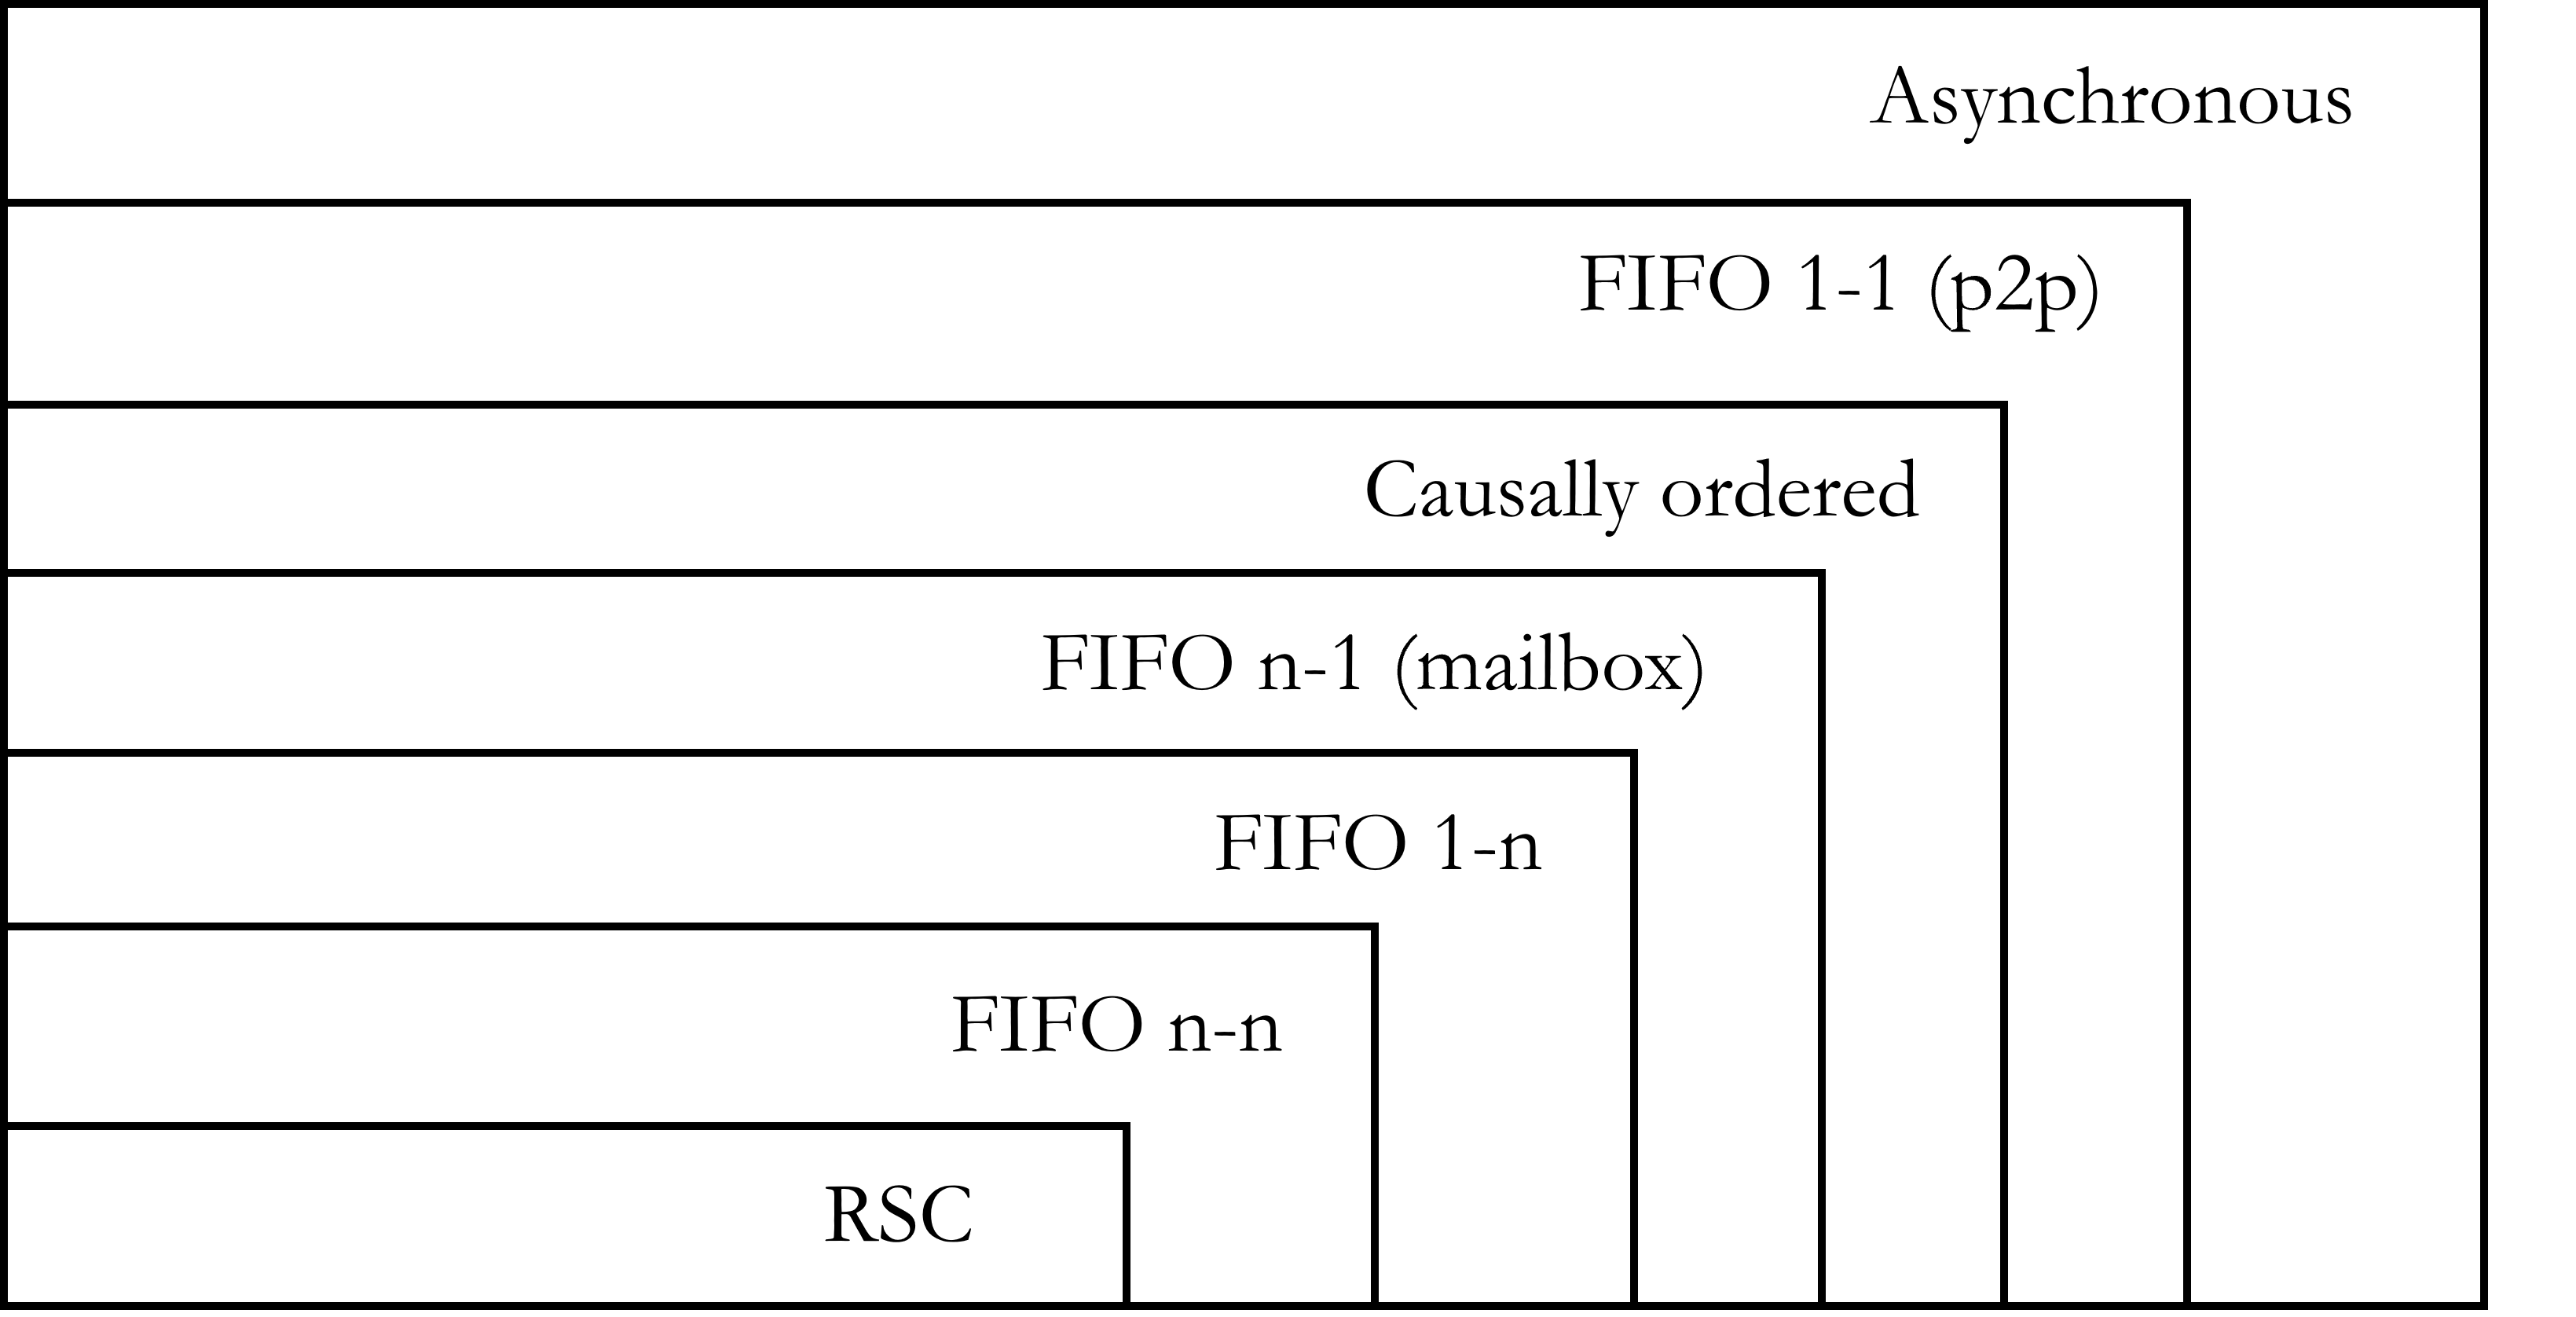
\includegraphics[width=8cm]{msc_hierarchy}
	\caption{The hierarchy of MSC classes.}
	\label{fig:msc_hierarchy}
\end{figure}

\subsection{Monadic Second-Order Logic}

The set of MSO formulas over (asynchronous) MSCs (over $\Procs$ and $\Msg$) is given by the grammar
$
\phi ::= true \mid x \procrel y \mid x \lhd y \mid \lambda(x) = a \mid x = y \mid x \in X \mid \exists x.\phi \mid \exists X.\phi \mid \phi \vee \phi \mid \neg \phi
$,
where $a \in \Act$, $x$ and $y$ are first-order variables, interpreted as
events of an MSC, and $X$ is a second-order variable, interpreted
as a set of events. We assume that we have an infinite supply of variables,
and we use common abbreviations such as $\wedge$, $\Rightarrow$, $\forall$, etc.
The satisfaction relation is defined in the standard way and self-explanatory.
For example, the formula $\neg\exists x.(\bigvee_{a \in \sAct} \lambda(x) = a \;\wedge\; \neg \mathit{matched}(x))$
with $\mathit{matched}(x) = \exists y.x \lhd y$
says that there are no unmatched send events.
It is not satisfied by  MSC $\mscweakuniver$
of Fig.~\ref{fig:msc_weak_univer},
as message $\msg_1$ is not received,
but by $\mscstrongexist$ from Fig.~\ref{fig:msc_strong_exist}.

Given a sentence $\phi$, i.e., a formula without free variables,
we let $L(\phi)$ denote the set of MSCs that satisfy $\phi$. Since we have defined the set of MSO formulas over asynchronous MSCs, the formula $\asformula = true$ clearly describes the set of asynchronous MSCs, i.e. $L(\asformula) = \asMSCs$. It is worth mentioning that the (reflexive) transitive closure of a binary relation defined by an MSO formula\footnote{See Section~\ref{sec:mso_extra} for details.} with free variables $x$ and $y$, such as $x \procrel y$, is MSO-definable so that the logic can freely use formulas of the form $x \procrel^+ y$, $x \procrel^* y$ or $x \le y$ (where $\le$ is interpreted as $\le_\msc$ for the given MSC $\msc$).

\paragraph*{Peer-to-peer MSCs}
	The set of \pp MSCs is MSO-definable as
	\[
		\ppformula = \neg \exists s.\exists s'. \left(
		\bigvee_{\substack{p \in \Procs, q \in \Procs}}\;
		\bigvee_{\substack{a,b \in \pqsAct{p}{q}}}\hspace{-1em}
		(\lambda(s) = a \;\wedge\; \lambda(s') = b) \;\wedge\; s \procrel^+ s' \;\wedge\;
		(\psi_1 \vee \psi_2 ) 	
		\right)
	\]
	where $\psi_1$ and $\psi_2$ are
	\[
		\psi_1 = \exists r.\exists r'.\left(
		\begin{array}{ll}
			s \lhd r & \wedge\\
			s' \lhd r' & \wedge\\
			r' \procrel^+ r &
		\end{array} 
		\right) \quad \quad
		\psi_2 = (\neg \mathit{matched}(s) \wedge \mathit{matched}(s'))
		\]
		\[
		matched(x) = \exists y. x \lhd y
	\]

The property $\ppformula$ says that there cannot be two matched send events $s$ and $s'$, with the same sender and receiver, such that either
\begin{enumerate*}[label={(\roman*)}]
	\item $s \procrel^+ s$ and their receipts happen in the reverse order, or
	\item $s$ is unmatched and $s'$ is matched.
\end{enumerate*}
In other words, it ensures that channels operate in FIFO mode, where an unmatched messages blocks the receipt of all the subsequent messages on that channel.
The set $\ppMSCs$ is therefore MSO-definable as $\ppMSCs=L(\ppformula)$.

\paragraph*{Causally ordered MSCs}
Given an MSC $\msc$, it is causally ordered if it satisfies the MSO formula
\[
	\coformula = \neg \exists s.\exists s'. \left(
	\bigvee_{\substack{q \in \Procs}}\;
	\bigvee_{\substack{a,b \in \pqsAct{\plh}{q}}}\hspace{-1em}
	(\lambda(s) = a \;\wedge\; \lambda(s') = b) \;\wedge\; s \le_\msc s' \;\wedge\;
	(\psi_1 \vee \psi_2 ) 	
	\right)
\]
where $\psi_1$ and $\psi_2$ are the same formulas used for \pp.

The property $\coformula$ says that there cannot be two send events $s$ and $s'$, with the same recipient, such that $s \le_\msc s'$ and either
\begin{enumerate*}[label={(\roman*)}]
	\item their corresponding receive events $r$ and $r'$ happen in the opposite order, i.e. $r' \procrel^+ r$, or
	\item $s$ is unmatched and $s'$ is matched.
\end{enumerate*}
The set $\coMSCs$ of causally ordered MSCs is therefore MSO-definable as $\coMSCs=L(\coformula)$.

\paragraph*{Mailbox MSCs}

Given an MSC $\msc$, it is a mailbox MSC if it satisfies the MSO formula
\[
	\mbformula = \ppformula \;\wedge\; \neg \exists x.\exists y.(\neg (x = y) \wedge x \preceq_\msc y \wedge y \preceq_\msc x)
\]
The set $\mbMSCs$ of mailbox MSCs is therefore MSO-definable as $\mbMSCs=L(\mbformula)$.
\davide{This does not match my definition of mailbox MSC, should I also give the alternative definition (the one in the concur paper) or rewrite everything according to my definition? Give both definitions and prove that they are equivalent}

\paragraph*{$\onen$ MSCs}

Given an MSC $\msc$, it is a $\onen$ MSC if it satisfies the MSO formula
\[
	\onenformula = \neg \exists x.\exists y.(\neg (x = y) \wedge x \lessdot_\msc y \wedge y \lessdot_\msc x)
\]
Here, $x \lessdot_\msc y$ is the MSO-definable transitive closure of the union of the MSO-definable relations $\procrel$, $\lhd$, and $\onenrel_\msc$. In particular, we can define $x \onenrel_\msc y$ as 
\[
x \onenrel_\msc y =
\begin{array}{rl}
& \left(
	\bigvee_{\substack{p \in \Procs\\a,b \in \psAct{p}}}\hspace{-1em}
	(\lambda(x) = a \;\wedge\; \lambda(y) = b)
	\;\wedge\; \mathit{matched}(x) \;\wedge\; \neg \mathit{matched}(y)
\right) \;\vee\\
& \left(
	\bigvee_{\substack{p \in \Procs\\a,b \in \prAct{p}}}\hspace{-1em}
	(\lambda(x) = a \;\wedge\; \lambda(y) = b)
	\;\wedge\; 
	\exists x'.\exists y'. (x' \lhd x \;\wedge\; y' \lhd y \;\wedge\; x' \procrel^+ y')
\right)\\
\end{array}
\]
The MSO formula for $x \onenrel_\msc y$ closely follows Definition~\ref{def:one_n_alt}. The set $\onenMSCs$ of mailbox MSCs is therefore MSO-definable as $\onenMSCs=L(\onenformula)$.

\paragraph*{$\nn$ MSCs}


\subsection{Existentially bounded MSCs}

\davidequestion{Should we say for all sends, also unmatched? Shouldn't it be $<$ instead of $\le$?}
\begin{definition}\label{def:lin_k_bounded}
	Let $\msc = (\Events,\procrel,\lhd,\lambda) \in \MSCs$ and $k \in \N$.
	A linearization $\linrel$ of $\msc$ is called
	$k$-\emph{bounded} if, for all $e \in \Matched{\msc}$, with $\lambda(e) = \sact{p}{q}{\msg}$, we have 
	\[
	\sametype{e}{\pqsAct{p}{q}}{\linrel} - \sametype{e}{\pqrAct{p}{q}}{\linrel} \le k.
	\]
\end{definition}
\noindent Recall that $\sametype{e}{\pqsAct{p}{q}}{\linrel}$ denotes the number of send events from $p$ to $q$ that occured before $e$, according to $\linrel$. Intuitively, a linearization is $k$-bounded if, at any moment in time, there are no more than $k$ messages in any channel.

\begin{definition}[Existentially bounded MSC]\label{def:ek_bounded_msc}
	Let $\msc = (\Events, \rightarrow, \lhd, \lambda) \in \asMSCs$ and $k \in \mathbb{N}$. We call $\msc$ \emph{existentially $k$-bounded} if it has a $k$-bounded linearization.
\end{definition}
Let $\asEk$ be the set of existentially $k$-bounded MSCs, for a given $k \in \N$.
\begin{definition}
	An MSC $\msc$ is \emph{\pp existentially $k$-bounded} (\pp-$\exists k$-bounded) if it is a \pp MSC and it is also existentially $k$-bounded.
\end{definition}
\begin{definition}
	An MSC $\msc$ is \emph{causally orderered existentially $k$-bounded} ($\cosymb$-$\exists k$-bounded) if it is a causally ordered MSC and it is also existentially $k$-bounded.
\end{definition}
When moving on to mailbox MSCs, the definition of mailbox existentially $k$-bounded MSC should require that there exists a $k$-bounded linearization that is also a mailbox linearization, not just any linearization. Recall that an MSC is a mailbox MSC if it has at least one mailbox linearization, which represents a sequence of events that can be executed by a mailbox system. Following this intuition, we want one of these mailbox linearizations to be $k$-bounded, because \emph{non}-mailbox linearizations cannot be executed by a mailbox system.
\begin{definition}
	An MSC $\msc$ is \emph{mailbox existentially $k$-bounded} (mb-$\exists k$-bounded) if it is a mailbox MSC and it has a $k$-bounded mailbox linearization.
\end{definition}
\davide{This paragraph depends on how we choose to formally define the mailbox communication model... we could go for a (i) single incoming channel, or (ii) just an enforcing of the delivery of messages by the transport layer.}
It should be noted that, for a $k$-bounded mailbox linearization, it is not necessarily true that at any time we have at most $k$ messages in each channel. Recall that in the mailbox communication architecture every process has a single incoming channel, but the Definition~\ref{def:lin_k_bounded} of $k$-bounded linearization considers the number of pending messages between each pair $(p,q)$ of processes. Let $n$ be the number of processes. We can say that, for a $k$-bounded mailbox linearization, we have at most $k(n-1)$ messages in each channel at any moment (because each process can have at most $k$ pending messages coming from any of the other $n-1$ processes).
\davide{An example would be nice.}

\begin{definition}
	An MSC $\msc$ is \emph{$\onen$ existentially $k$-bounded} (1n-$\exists k$-bounded) if it is a $\onen$ MSC and it has a $k$-bounded $\onen$ linearization.
\end{definition}

\subsubsection{MSO-definability}

In this section, we will investigate the MSO-definability of all the variants of existentially $k$-bounded MSCs that we introduced. Following the approach taken in \cite{DBLP:conf/fossacs/LohreyM02}, we introduce a binary relation $\relb$ ($\linrel_b$ in their work) associated with a given bound $k$ and an MSC $\msc$. Let $k \ge 1$ and $\msc$ be a fixed MSC: we have $r \relb s$ if, for some $i \ge 1$ and some channel ($p$,$q$)\footnote{Recall that ($p,\,q$) is a channel where messages are sent by $p$ and received by $q$.}:
\begin{enumerate}\itemsep=0.5ex
	\item $r$ is the $i$-th receive event (executed by $q$).
	\item $s$ is the ($i+k$)-th send event (executed by $p$).
\end{enumerate} 
Note that, for any two events $s$ and $r$ such that $r \relb s$, every linearization of $\msc$ in which $r$ is executed after $s$ cannot $k$-bounded. Intuitively, we can read $r \relb s$ as "$r$ has to be executed before $s$ in a $k$-bounded linearization".\davidequestionsmall{Should I prove it?} A linearization $\linrel$ that respects $\relb$ (i.e. $\relb \,\subseteq\, \linrel$) is $k$-bounded.\davide{An example would be nice.} In \cite{DBLP:conf/fossacs/LohreyM02} it was shown that an MSC is existentially $k$-bounded if and only if the relation $\le_\msc \cup \relb$ is acyclic\footnote{A binary relation is acyclic if it does not contain a "cycle", which is to say its transitive closure is antisymmetric.}. Since $\le_\msc$ and acyclicity are both MSO-definable (we did not show the latter), it suffices to find an MSO formula that defines the $\relb$ relation to say that the set of existentially $k$-bounded MSCs is MSO-definable. In particular, we can define $r \relb s$ as
\davidequestion{This is not valid for asynchronous, it is for \pp, but it might need some tweaking depending on if we want to count or not unmatched messages}
\[
r \relb s=\exists s_1.\exists s_2.\dots.\exists s_k.\left(
allSend\_p\_q
\;\wedge\; s_1\procrel s_2\procrel\dots
\procrel s_k\procrel s
\;\wedge\; s_1 \lhd r
\right)
\]
where $allSend\_p\_q$ checks if $s,s_1,\dots,s_k$ are all send events from and to the same process (i.e., on the same channel)
\[
allSend\_p\_q=
\bigvee_{\substack{p \in \Procs, q \in \Procs}}\;
\bigwedge_{e \in {s, s_1, ..., s_k}}\;
\bigvee_{a \in \pqsAct{p}{q}}\;
\lambda(e) = a
\]
It follows that, given $k \in \N$, the set of existentially $k$-bounded MSCs is MSO-definable. Causally ordered and \pp existentially $k$-bounded MSCs are clearly MSO-definable by definition, since we already showed that \pp MSCs, causally ordered MSCs, and existentially $k$-bounded MSCs are all MSO-definable. The set of mailbox existentially $k$-bounded MSCs was already shown to be MSO-definable in \cite{DBLP:conf/concur/BolligGFLLS21}, but they use a slightly different definition of mailbox existentially $k$-bounded MSC. With their definition, a $\exists k$-mb-bounded MSC has at most $k$ messages in any incoming channel at any moment, whereas according to our definition the threshold is $k(n-1)$, were $n$ is the number of processes. In particular, they introduce a binary relation $\revb \,\supseteq\, \relb$ and they show that an MSC $\msc$ is $\exists k$-mb-bounded iff $\preceq_\msc \cup \revb$ is acyclic. With our definition, an MSC is $\exists k$-mb-bounded iff $\preceq_\msc \cup \relb$ is acyclic. \davidequestionsmall{Should I rewrite the proof?}This can easily be shown by simply replacing $\revb$ with $\relb$ in the proof given in \cite{DBLP:conf/concur/BolligGFLLS21}. We already talked about the MSO-defininability of $\preceq_\msc$, $\relb$, and acyclicity, so the set of mailbox existentially $k$-bounded MSCs is also MSO-definable.

\subsubsection{Special treewidth}

In \cite[Lemma 5.37]{DBLP:journals/corr/abs-1904-06942} it was shown that the special treewidth of existentially $k$-bounded MSCs is bounded by $k\,|\Procs|^2$, for $k \ge 1$. Actually, STW-boundness was shown for the more general $\mathsf{CBM}$ class (Concurrent Behaviours with Matching), but the result is still valid since $\asMSCs \subset \mathsf{CBM}$. \davidequestionsmall{Should I rewrite the proof more clearly?} The special treewidth of both \pp-$\exists k$-bounded and $\cosymb$-$\exists k$-bounded MSCs is also bounded, since every \pp or causally ordered existentially $k$-bounded MSC is existentially $k$-bounded by definition. Similarly, mb-$\exists k$-bounded MSCs have also a bounded special treewidth, since it is trivial to see that every existentially mailbox $k$-bounded MSC is existentially $k$-bounded.

\subsection{Universally bounded MSCs}

\begin{definition}[Universally bounded MSC]\label{def:uk_bounded_msc}
	Let $\msc = (\Events, \rightarrow, \lhd, \lambda) \in \asMSCs$ and $k \in \mathbb{N}$. We call $\msc$ \emph{universally $k$-bounded} if all of its linearizations are $k$-bounded.
\end{definition}
Let $\asUk$ be the set of universally $k$-bounded MSCs.
\begin{definition}
	An MSC $\msc$ is \emph{\pp universally $k$-bounded} (\pp-$\forall k$-bounded) if it is a \pp MSC and it is also universally $k$-bounded.
\end{definition}
Let $\ppUk$ be the set of \pp universally $k$-bounded MSCs.
\begin{definition}
	An MSC $\msc$ is \emph{causally orderered universally $k$-bounded} ($\cosymb$-$\forall k$-bounded) if it is a causally ordered MSC and it is also universally $k$-bounded.
\end{definition}
Let $\coUk$ be the set of causally ordered universally $k$-bounded MSCs.
\begin{definition}
	An MSC $\msc$ is \emph{mailbox universally $k$-bounded} (mb-$\forall k$-bounded) if it is a mailbox MSC and all of its mailbox linearizations are $k$-bounded.
\end{definition}
Let $\mbUk$ be the set of mailbox universally $k$-bounded MSCs.
\begin{definition}
	An MSC $\msc$ is \emph{$\onen$ universally $k$-bounded} (1n-$\forall k$-bounded) if it is a $\onen$ MSC and all of its $\onen$ linearizations are $k$-bounded.
\end{definition}
Let $\mbUk$ be the set of mailbox universally $k$-bounded MSCs.

\subsubsection{Hierarchy}

\davide{Investigate hierarchy of universally $k$-bounded MSCs.}
In this section we will investigate the relations between the various classes of universally $k$-bounded MSCs that we introduced. From their definition, it is quite straightforward to see that $\coUk \subseteq \ppUk \subseteq \asUk$. The set of mailbox universally $k$-bounded MSCs, however, does not fit in this hierarchy. Recall that an MSC is mb-$\forall k$-bounded if all of its mailbox linearizations are $k$-bounded, but the definition does not say anything about non-mailbox linearizations. It can be the case that an MSC has a bound $k$ for its mailbox linearizations, but a higher bound $k'$ for non-mailbox linearizations. Fig.~\ref{fig:mb_uk} shows an MSC $\msc$ which is mb-$\forall 1$-bounded, but $\forall 2$-bounded. According to the mailbox semantics, a mailbox linearization of $\msc$ has to respect the order $!m_1 \mbrel_\msc\, !m_3 \mbrel_\msc\, !m_4$. Note that all mailbox linearizations are $1$-bounded, but we are able to find a non-mailbox linearization that is 2-bounded, such as $!m_1 \linrel\, !m_4 \linrel\, ?m_1 \linrel\, !m_2 \linrel\, ?m_2 \linrel\, !m_3 \linrel\, !m_4 \linrel\, ?m_3 \linrel\, ?m_4$.

\begin{figure}[h]
\begin{center}
\begin{tikzpicture}
	\newproc{0}{p}{-1.9};
	\newproc{1}{q}{-1.9};
	\newproc{2}{r}{-1.9};

	\newmsgml{0}{1}{-0.5}{1}{0.5}{black};
	\newmsgml{1}{2}{-0.7}{2}{0.5}{black};
	\newmsgml{2}{1}{-1.2}{3}{0.5}{black};
	\newmsgml{0}{1}{-1.4}{4}{0.5}{black};
\end{tikzpicture}
\caption{Example of MSC which is mailbox universally 1-bounded, but not universally 1-bounded (it is universally 2-bounded).}
\label{fig:mb_uk}
\end{center}
\end{figure}

For a given $k \in \N$, Fig~\ref{fig:uk_hierarchy} gives a visual representation of how the diffent variants of universally $k$-bounded MSCs are related.

\begin{figure}[h]
	\centering
	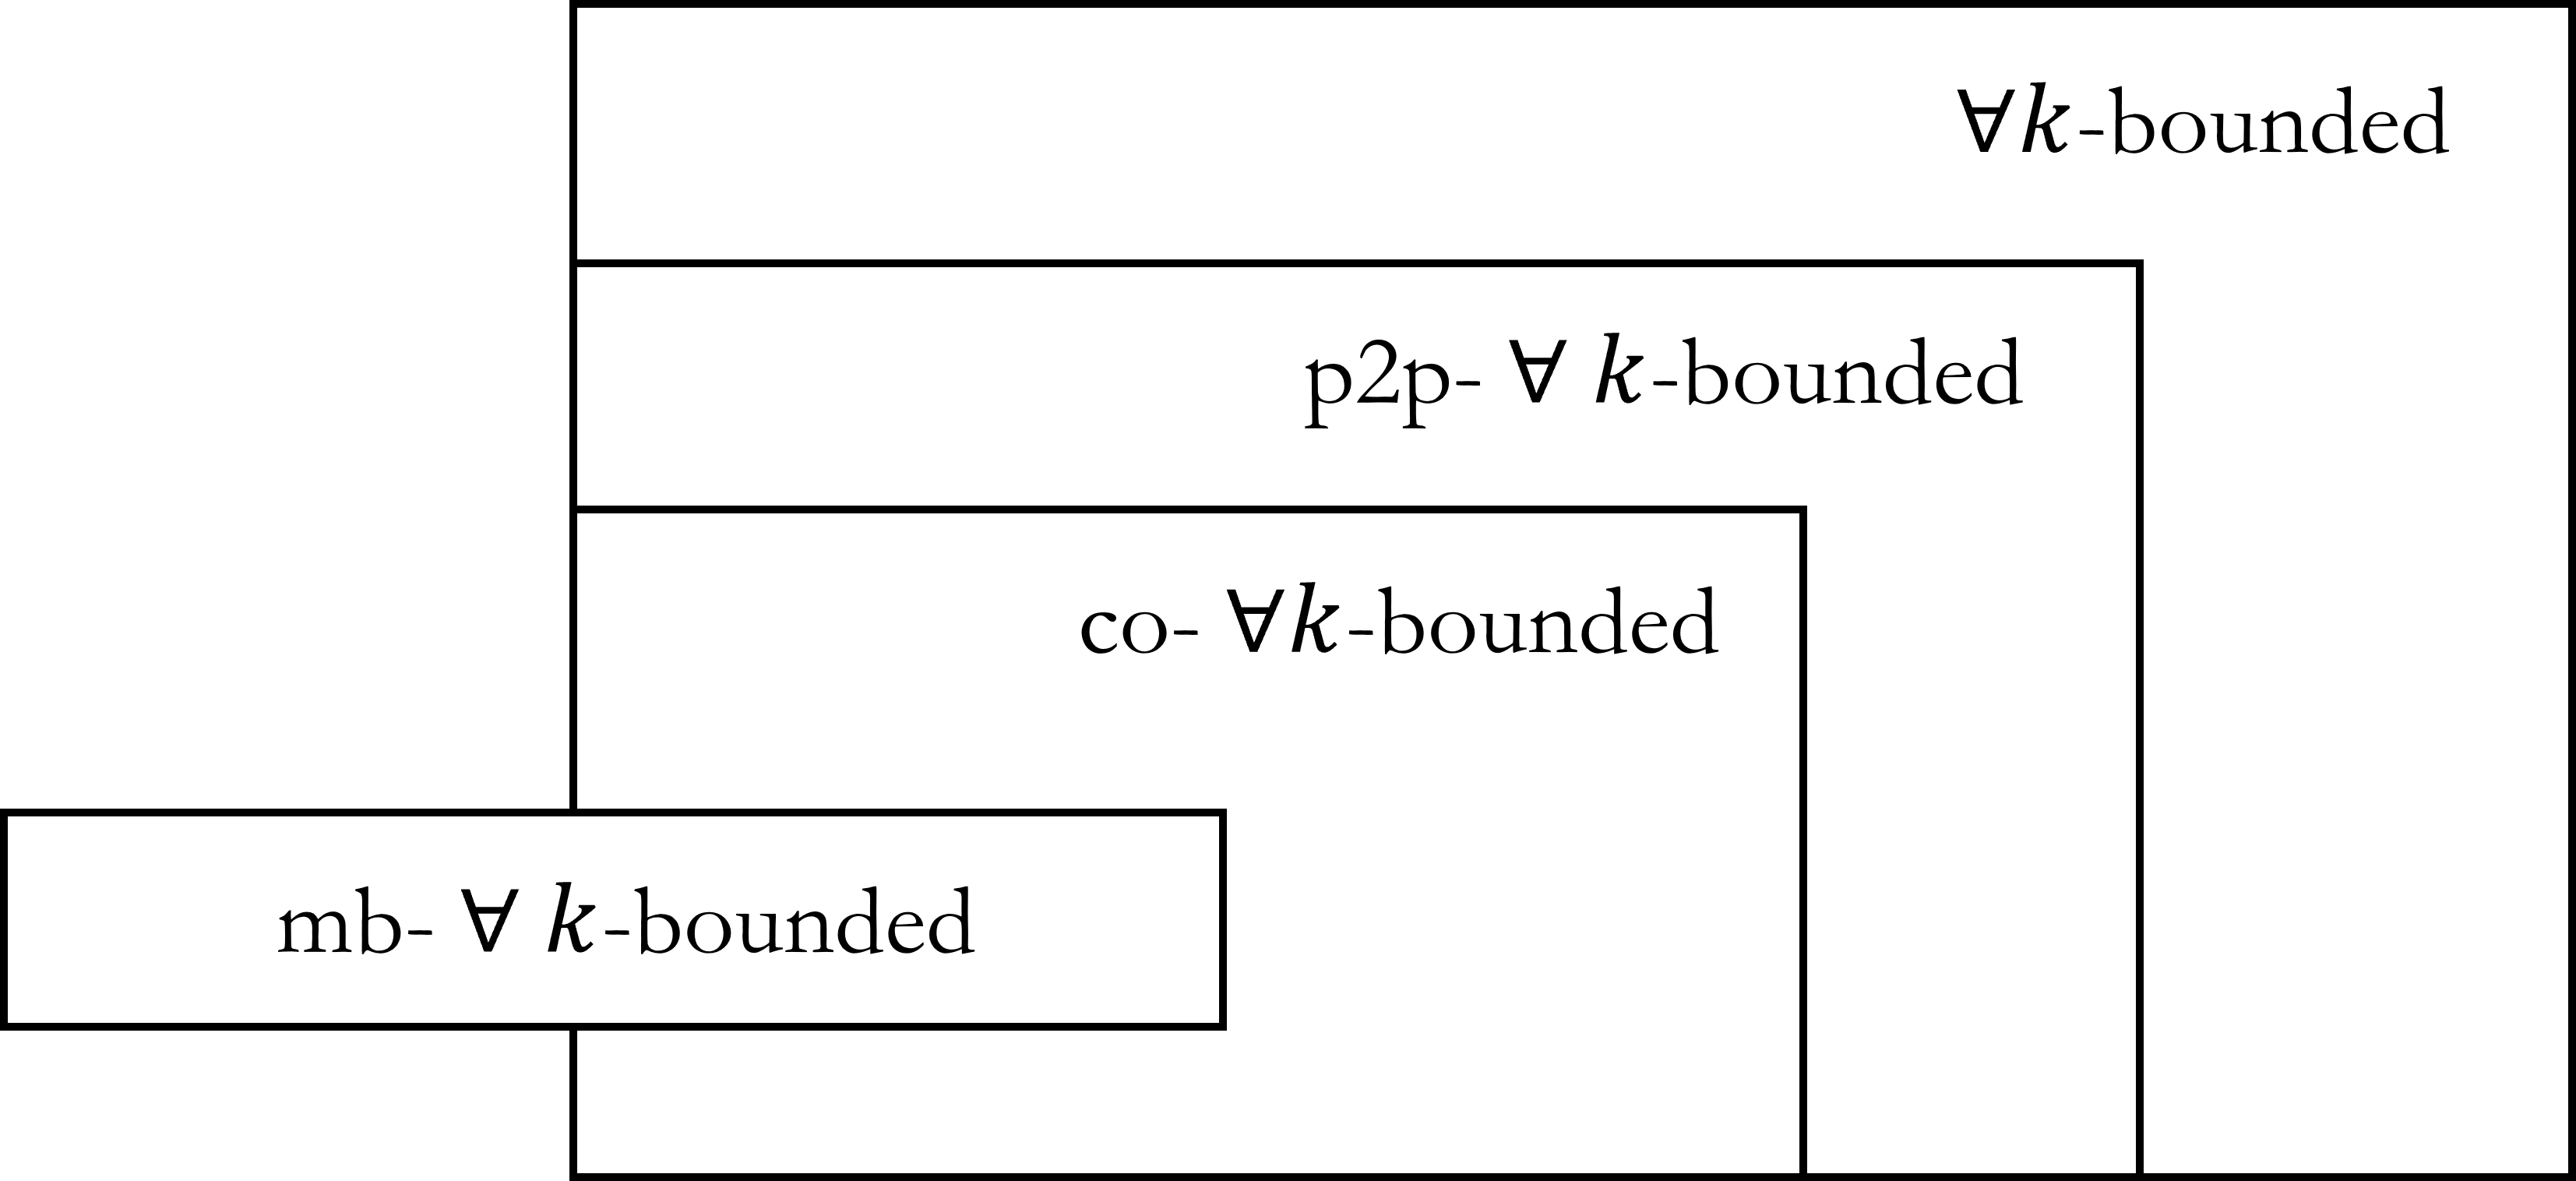
\includegraphics[width=8cm]{uni_k_hierarchy.png}
	\caption{The relation between different variants of universally $k$-bounded MSCs, given a $k \in \N$.}
	\label{fig:uk_hierarchy}
\end{figure}

\subsubsection{MSO-definability}

In this section, we will investigate the MSO-definability of all the variants of universally $k$-bounded MSCs that we introduced.

In \cite{DBLP:conf/fossacs/LohreyM02}, it is shown that an MSC $\msc$ is universally $k$-bounded if and only if $\relb \;\subseteq\; \le_\msc$. In other words, $r \relb s \Rightarrow r \le_\msc s$ for any two events $r$ and $s$. This is equivalent to saying that every linearization $\linrel$ of $\msc$ respects the $\relb$ relation, since $\relb \;\subseteq\; \le_\msc \;\subseteq\; \linrel$. We already showed that $\relb$ is MSO-definable. The MSO formula that defines universally $k$-bounded  MSCs can be written as
\[ \asUkformula = \neg \exists r.\exists s.(r \relb s \wedge \neg(r \le_\msc s)) \]
Causally ordered and \pp universally $k$-bounded MSCs are clearly MSO-definable by definition, since we already showed that \pp MSCs, causally ordered MSCs, and universally $k$-bounded MSCs are all MSO-definable. To show MSO-definability of mailbox universally $k$-bounded MSCs we first prove the following property.

\begin{proposition}\label{prop:mb_ukb_alt}
	An MSC $\msc$ is mailbox universally $k$-bounded if and only if $\relb \;\subseteq\; \preceq_\msc$.
\end{proposition}
\begin{proof}
	Consider an MSC $\msc$ and a $k \in \N$.\newline
	($\Leftarrow$) Suppose $\relb \;\subseteq\; \preceq_\msc$. For every mailbox linearization $\mblinrel$ of $\msc$ we have that $\preceq_\msc \;\subseteq\; \mblinrel$. This implies $\relb \;\subseteq\; \mblinrel$, that is to say every mailbox linearization is $k$-bounded.\newline
	($\Rightarrow$) Suppose $\msc$ is a mailbox universally $k$-bounded MSC. By definition, every mailbox linearization $\mblinrel$ of $\msc$ is $k$-bounded, i.e. $\relb \;\subseteq\; \mblinrel$, and we have $\preceq_\msc \;\subseteq\; \mblinrel$, according to the definition of mailbox linearization. Moreover, we also know that $\preceq_\msc \cup \relb$ is acyclic, since $\msc$ is existentially $k$-bounded\footnote{Every mailbox universally $k$-bounded MSC is also a mailbox existentially $k$-bounded MSC by definition.}. Suppose now, by contradiction, that $\relb \;\nsubseteq\; \preceq_\msc$. Thus, there must be at least two events $r$ and $s$ such that $r \relb s$ and $r \npreceq_\msc s$; we also have $s \npreceq_\msc r$ because of the acyclicity of $\preceq_\msc \cup \relb$ (we cannot have the cycle $r \relb s \preceq_\msc r$). Consider a mailbox linearization $\mblinrel$  of $\msc$, such that $s \mblinrel r$. Note that such a mailbox linearization always exists, since $r$ and $s$ are incomparable w.r.t. the partial order $\preceq_\msc$ (i.e. $s \npreceq_\msc r$)\footnote{If two elements $a$ and $b$ of a set are incomparable w.r.t. a partial order $\le$, it is always possible to find a total order of the elements (that respects $\le$) where $a$ comes before $b$, or viceversa.}. This mailbox linearization does not respect $\relb$ (because we have $s \mblinrel r$ and $r \relb s$), so it is not $k$-bounded. This is a contradiction, since we assumed that $\msc$ was a mailbox universally $k$-bounded MSC. It has to be that $\relb \subseteq \preceq_\msc$.
\end{proof}

Using Proposition~\ref{prop:mb_ukb_alt}, we can now easily write the MSO formula that defines mailbox universally $k$-bounded MSCs as
\[ \mbUkformula = \neg \exists r.\exists s.(r \relb s \wedge \neg(r \preceq_\msc s)) \]

\subsubsection{Special treewidth}

All the variants of universally $k$-bounded MSCs that we presented have a bounded special treewidth. This directly follows from the STW-boundness of the existential counterparts, since every universally $k$-bounded MSC is existentially $k$-bounded by definition.

\subsubsection{MSO additional content}\label{sec:mso_extra}

\davide{Show MSO-definability of the transitive closure of a binary relation.}

\paragraph*{Acyclicity} 

Given a binary relation $\to$, the acyclicity of $\to$ can be expressed with an MSO formula. Recall that, given a binary relation $\to$, it is acyclic if and only if its transitive closure $\to^*$ is antisymmetric. The MSO formula of acyclicity directly follows from this definition:
\[
\Phi_{acyclic} =  \neg \exists x.\exists y.(x \to^* y \;\wedge\; y \to^* x).   
\]
\input{extra/proofs_extra.tex}

\printbibliography

\end{document}